\documentclass[1p]{elsarticle_modified}
%\bibliographystyle{elsarticle-num}

%\usepackage[colorlinks]{hyperref}
%\usepackage{abbrmath_seonhwa} %\Abb, \Ascr, \Acal ,\Abf, \Afrak
\usepackage{amsfonts}
\usepackage{amssymb}
\usepackage{amsmath}
\usepackage{amsthm}
\usepackage{scalefnt}
\usepackage{amsbsy}
\usepackage{kotex}
\usepackage{caption}
\usepackage{subfig}
\usepackage{color}
\usepackage{graphicx}
\usepackage{xcolor} %% white, black, red, green, blue, cyan, magenta, yellow
\usepackage{float}
\usepackage{setspace}
\usepackage{hyperref}

\usepackage{tikz}
\usetikzlibrary{arrows}

\usepackage{multirow}
\usepackage{array} % fixed length table
\usepackage{hhline}

%%%%%%%%%%%%%%%%%%%%%
\makeatletter
\renewcommand*\env@matrix[1][\arraystretch]{%
	\edef\arraystretch{#1}%
	\hskip -\arraycolsep
	\let\@ifnextchar\new@ifnextchar
	\array{*\c@MaxMatrixCols c}}
\makeatother %https://tex.stackexchange.com/questions/14071/how-can-i-increase-the-line-spacing-in-a-matrix
%%%%%%%%%%%%%%%

\usepackage[normalem]{ulem}

\newcommand{\msout}[1]{\ifmmode\text{\sout{\ensuremath{#1}}}\else\sout{#1}\fi}
%SOURCE: \msout is \stkout macro in https://tex.stackexchange.com/questions/20609/strikeout-in-math-mode

\newcommand{\cancel}[1]{
	\ifmmode
	{\color{red}\msout{#1}}
	\else
	{\color{red}\sout{#1}}
	\fi
}

\newcommand{\add}[1]{
	{\color{blue}\uwave{#1}}
}

\newcommand{\replace}[2]{
	\ifmmode
	{\color{red}\msout{#1}}{\color{blue}\uwave{#2}}
	\else
	{\color{red}\sout{#1}}{\color{blue}\uwave{#2}}
	\fi
}

\newcommand{\Sol}{\mathcal{S}} %segment
\newcommand{\D}{D} %diagram
\newcommand{\A}{\mathcal{A}} %arc


%%%%%%%%%%%%%%%%%%%%%%%%%%%%%5 test

\def\sl{\operatorname{\textup{SL}}(2,\Cbb)}
\def\psl{\operatorname{\textup{PSL}}(2,\Cbb)}
\def\quan{\mkern 1mu \triangleright \mkern 1mu}

\theoremstyle{definition}
\newtheorem{thm}{Theorem}[section]
\newtheorem{prop}[thm]{Proposition}
\newtheorem{lem}[thm]{Lemma}
\newtheorem{ques}[thm]{Question}
\newtheorem{cor}[thm]{Corollary}
\newtheorem{defn}[thm]{Definition}
\newtheorem{exam}[thm]{Example}
\newtheorem{rmk}[thm]{Remark}
\newtheorem{alg}[thm]{Algorithm}

\newcommand{\I}{\sqrt{-1}}
\begin{document}

%\begin{frontmatter}
%
%\title{Boundary parabolic representations of knots up to 8 crossings}
%
%%% Group authors per affiliation:
%\author{Yunhi Cho} 
%\address{Department of Mathematics, University of Seoul, Seoul, Korea}
%\ead{yhcho@uos.ac.kr}
%
%
%\author{Seonhwa Kim} %\fnref{s_kim}}
%\address{Center for Geometry and Physics, Institute for Basic Science, Pohang, 37673, Korea}
%\ead{ryeona17@ibs.re.kr}
%
%\author{Hyuk Kim}
%\address{Department of Mathematical Sciences, Seoul National University, Seoul 08826, Korea}
%\ead{hyukkim@snu.ac.kr}
%
%\author{Seokbeom Yoon}
%\address{Department of Mathematical Sciences, Seoul National University, Seoul, 08826,  Korea}
%\ead{sbyoon15@snu.ac.kr}
%
%\begin{abstract}
%We find all boundary parabolic representation of knots up to 8 crossings.
%
%\end{abstract}
%\begin{keyword}
%    \MSC[2010] 57M25 
%\end{keyword}
%
%\end{frontmatter}

%\linenumbers
%\tableofcontents
%
\newcommand\colored[1]{\textcolor{white}{\rule[-0.35ex]{0.8em}{1.4ex}}\kern-0.8em\color{red} #1}%
%\newcommand\colored[1]{\textcolor{white}{ #1}\kern-2.17ex	\textcolor{white}{ #1}\kern-1.81ex	\textcolor{white}{ #1}\kern-2.15ex\color{red}#1	}

{\Large $\underline{12a_{0896}~(K12a_{0896})}$}

\setlength{\tabcolsep}{10pt}
\renewcommand{\arraystretch}{1.6}
\vspace{1cm}\begin{tabular}{m{100pt}>{\centering\arraybackslash}m{274pt}}
\multirow{5}{120pt}{
	\centering
	\includegraphics[width=112pt]{../../../GIT/diagram.site/Diagrams/png/1697_12a_0896.png}\\
\ \ \ A knot diagram\footnotemark}&
\allowdisplaybreaks
\textbf{Linearized knot diagam} \\
\cline{2-2}
 &
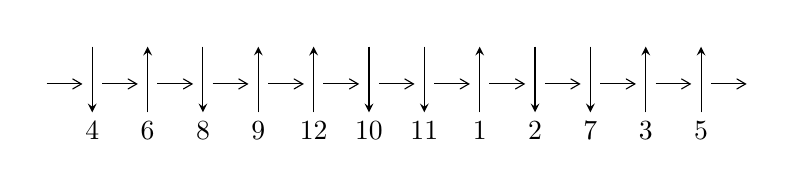
\begin{tikzpicture}[x=20pt, y=17pt]
	% nodes
	\node (C0) at (0, 0) {};
	\node (C1) at (1, 0) {};
	\node (C1U) at (1, +1) {};
	\node (C1D) at (1, -1) {4};

	\node (C2) at (2, 0) {};
	\node (C2U) at (2, +1) {};
	\node (C2D) at (2, -1) {6};

	\node (C3) at (3, 0) {};
	\node (C3U) at (3, +1) {};
	\node (C3D) at (3, -1) {8};

	\node (C4) at (4, 0) {};
	\node (C4U) at (4, +1) {};
	\node (C4D) at (4, -1) {9};

	\node (C5) at (5, 0) {};
	\node (C5U) at (5, +1) {};
	\node (C5D) at (5, -1) {12};

	\node (C6) at (6, 0) {};
	\node (C6U) at (6, +1) {};
	\node (C6D) at (6, -1) {10};

	\node (C7) at (7, 0) {};
	\node (C7U) at (7, +1) {};
	\node (C7D) at (7, -1) {11};

	\node (C8) at (8, 0) {};
	\node (C8U) at (8, +1) {};
	\node (C8D) at (8, -1) {1};

	\node (C9) at (9, 0) {};
	\node (C9U) at (9, +1) {};
	\node (C9D) at (9, -1) {2};

	\node (C10) at (10, 0) {};
	\node (C10U) at (10, +1) {};
	\node (C10D) at (10, -1) {7};

	\node (C11) at (11, 0) {};
	\node (C11U) at (11, +1) {};
	\node (C11D) at (11, -1) {3};

	\node (C12) at (12, 0) {};
	\node (C12U) at (12, +1) {};
	\node (C12D) at (12, -1) {5};
	\node (C13) at (13, 0) {};

	% arrows
	\draw[->,>={angle 60}]
	(C0) edge (C1) (C1) edge (C2) (C2) edge (C3) (C3) edge (C4) (C4) edge (C5) (C5) edge (C6) (C6) edge (C7) (C7) edge (C8) (C8) edge (C9) (C9) edge (C10) (C10) edge (C11) (C11) edge (C12) (C12) edge (C13) ;	\draw[->,>=stealth]
	(C1U) edge (C1D) (C2D) edge (C2U) (C3U) edge (C3D) (C4D) edge (C4U) (C5D) edge (C5U) (C6U) edge (C6D) (C7U) edge (C7D) (C8D) edge (C8U) (C9U) edge (C9D) (C10U) edge (C10D) (C11D) edge (C11U) (C12D) edge (C12U) ;
	\end{tikzpicture} \\
\hhline{~~} \\& 
\textbf{Solving Sequence} \\ \cline{2-2} 
 &
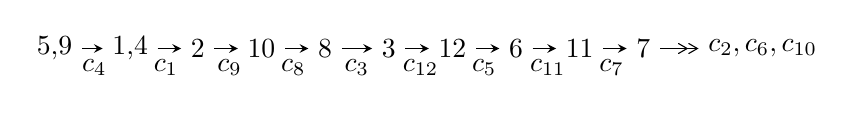
\begin{tikzpicture}[x=23pt, y=7pt]
	% node
	\node (A0) at (-1/8, 0) {5,9};
	\node (A1) at (17/16, 0) {1,4};
	\node (A2) at (17/8, 0) {2};
	\node (A3) at (25/8, 0) {10};
	\node (A4) at (33/8, 0) {8};
	\node (A5) at (41/8, 0) {3};
	\node (A6) at (49/8, 0) {12};
	\node (A7) at (57/8, 0) {6};
	\node (A8) at (65/8, 0) {11};
	\node (A9) at (73/8, 0) {7};
	\node (C1) at (1/2, -1) {$c_{4}$};
	\node (C2) at (13/8, -1) {$c_{1}$};
	\node (C3) at (21/8, -1) {$c_{9}$};
	\node (C4) at (29/8, -1) {$c_{8}$};
	\node (C5) at (37/8, -1) {$c_{3}$};
	\node (C6) at (45/8, -1) {$c_{12}$};
	\node (C7) at (53/8, -1) {$c_{5}$};
	\node (C8) at (61/8, -1) {$c_{11}$};
	\node (C9) at (69/8, -1) {$c_{7}$};
	\node (A10) at (11, 0) {$c_{2},c_{6},c_{10}$};

	% edge
	\draw[->,>=stealth]	
	(A0) edge (A1) (A1) edge (A2) (A2) edge (A3) (A3) edge (A4) (A4) edge (A5) (A5) edge (A6) (A6) edge (A7) (A7) edge (A8) (A8) edge (A9) ;
	\draw[->>,>={angle 60}]	
	(A9) edge (A10);
\end{tikzpicture} \\ 

\end{tabular} \\

\footnotetext{
The image of knot diagram is generated by the software ``\textbf{Draw programme}" developed by Andrew Bartholomew(\url{http://www.layer8.co.uk/maths/draw/index.htm\#Running-draw}), where we modified some parts for our purpose(\url{https://github.com/CATsTAILs/LinksPainter}).
}\phantom \\ \newline 
\centering \textbf{Ideals for irreducible components\footnotemark of $X_{\text{par}}$} 
 
\begin{align*}
I^u_{1}&=\langle 
-1.34885\times10^{51} u^{44}-9.18014\times10^{50} u^{43}+\cdots+1.51382\times10^{51} b+5.69474\times10^{50},\;a-1,\\
\phantom{I^u_{1}}&\phantom{= \langle  }u^{45}+u^{44}+\cdots+u^2+1\rangle \\
I^u_{2}&=\langle 
-3.32331\times10^{380} u^{89}+1.05242\times10^{381} u^{88}+\cdots+6.08883\times10^{382} b+3.39083\times10^{385},\\
\phantom{I^u_{2}}&\phantom{= \langle  }4.71676\times10^{505} u^{89}-6.33964\times10^{505} u^{88}+\cdots+1.97874\times10^{507} a-1.81413\times10^{510},\\
\phantom{I^u_{2}}&\phantom{= \langle  }u^{90}+16 u^{88}+\cdots+27804 u+13223\rangle \\
I^u_{3}&=\langle 
-3.69959\times10^{18} u^{30}+9.95612\times10^{17} u^{29}+\cdots+5.38462\times10^{18} b-7.23401\times10^{18},\;a+1,\\
\phantom{I^u_{3}}&\phantom{= \langle  }u^{31}+7 u^{29}+\cdots+5 u-1\rangle \\
I^u_{4}&=\langle 
4 u^5+6 u^4- u^3-20 u^2+7 b+2 u+1,\;2 u^5+3 u^4+3 u^3-3 u^2+7 a+u-17,\;u^6+u^5- u^4-4 u^3+3 u^2-1\rangle \\
I^u_{5}&=\langle 
- u^2+b,\;a-1,\;u^3- u^2+1\rangle \\
\\
\end{align*}
\raggedright * 5 irreducible components of $\dim_{\mathbb{C}}=0$, with total 175 representations.\\
\footnotetext{All coefficients of polynomials are rational numbers. But the coefficients are sometimes approximated in decimal forms when there is not enough margin.}
\newpage
\renewcommand{\arraystretch}{1}
\centering \section*{I. $I^u_{1}= \langle -1.35\times10^{51} u^{44}-9.18\times10^{50} u^{43}+\cdots+1.51\times10^{51} b+5.69\times10^{50},\;a-1,\;u^{45}+u^{44}+\cdots+u^2+1 \rangle$}
\flushleft \textbf{(i) Arc colorings}\\
\begin{tabular}{m{7pt} m{180pt} m{7pt} m{180pt} }
\flushright $a_{5}=$&$\begin{pmatrix}1\\0\end{pmatrix}$ \\
\flushright $a_{9}=$&$\begin{pmatrix}0\\u\end{pmatrix}$ \\
\flushright $a_{1}=$&$\begin{pmatrix}1\\0.891028 u^{44}+0.606424 u^{43}+\cdots+1.18246 u-0.376185\end{pmatrix}$ \\
\flushright $a_{4}=$&$\begin{pmatrix}1\\u^2\end{pmatrix}$ \\
\flushright $a_{2}=$&$\begin{pmatrix}-0.891028 u^{44}-0.606424 u^{43}+\cdots-1.18246 u+1.37618\\1.21699 u^{44}+0.887098 u^{43}+\cdots+2.07349 u-0.660788\end{pmatrix}$ \\
\flushright $a_{10}=$&$\begin{pmatrix}0.637367 u^{44}+0.854223 u^{43}+\cdots+2.26087 u+0.274666\\-0.967895 u^{44}-1.55698 u^{43}+\cdots-3.27442 u-1.38255\end{pmatrix}$ \\
\flushright $a_{8}=$&$\begin{pmatrix}- u\\0.284603 u^{44}+0.610564 u^{43}+\cdots+1.37618 u+0.891028\end{pmatrix}$ \\
\flushright $a_{3}=$&$\begin{pmatrix}0.325961 u^{44}+0.280673 u^{43}+\cdots+0.891028 u+0.715397\\0.0822486 u^{44}+0.0152712 u^{43}+\cdots-0.0512955 u-0.592079\end{pmatrix}$ \\
\flushright $a_{12}=$&$\begin{pmatrix}-0.891028 u^{44}-0.606424 u^{43}+\cdots-1.18246 u+1.37618\\0.891028 u^{44}+0.606424 u^{43}+\cdots+1.18246 u-0.376185\end{pmatrix}$ \\
\flushright $a_{6}=$&$\begin{pmatrix}0.513771 u^{44}-0.317623 u^{43}+\cdots+0.304119 u-2.06785\\-1.40480 u^{44}-0.288801 u^{43}+\cdots-1.48658 u+3.44403\end{pmatrix}$ \\
\flushright $a_{11}=$&$\begin{pmatrix}-0.547463 u^{44}-0.224911 u^{43}+\cdots+0.274234 u+0.710542\\0.0683607 u^{44}-0.240991 u^{43}+\cdots-0.677215 u-0.00789983\end{pmatrix}$ \\
\flushright $a_{7}=$&$\begin{pmatrix}0.0291410 u^{44}+0.0929449 u^{43}+\cdots+0.162826 u+0.628549\\-0.547462 u^{44}-0.504253 u^{43}+\cdots-1.14241 u+0.332842\end{pmatrix}$\\&\end{tabular}
\flushleft \textbf{(ii) Obstruction class $= -1$}\\~\\
\flushleft \textbf{(iii) Cusp Shapes $= 1.86191 u^{44}-0.722513 u^{43}+\cdots-3.52946 u-9.43826$}\\~\\
\newpage\renewcommand{\arraystretch}{1}
\flushleft \textbf{(iv) u-Polynomials at the component}\newline \\
\begin{tabular}{m{50pt}|m{274pt}}
Crossings & \hspace{64pt}u-Polynomials at each crossing \\
\hline $$\begin{aligned}c_{1}\end{aligned}$$&$\begin{aligned}
&u^{45}-38 u^{44}+\cdots+6130 u-359
\end{aligned}$\\
\hline $$\begin{aligned}c_{2},c_{11}\end{aligned}$$&$\begin{aligned}
&u^{45}+10 u^{43}+\cdots+20 u+1
\end{aligned}$\\
\hline $$\begin{aligned}c_{3},c_{9}\end{aligned}$$&$\begin{aligned}
&u^{45}-2 u^{44}+\cdots-40 u-29
\end{aligned}$\\
\hline $$\begin{aligned}c_{4},c_{8}\end{aligned}$$&$\begin{aligned}
&u^{45}- u^{44}+\cdots- u^2-1
\end{aligned}$\\
\hline $$\begin{aligned}c_{5},c_{12}\end{aligned}$$&$\begin{aligned}
&u^{45}-31 u^{44}+\cdots-294912 u+16384
\end{aligned}$\\
\hline $$\begin{aligned}c_{6},c_{7},c_{10}\end{aligned}$$&$\begin{aligned}
&u^{45}+14 u^{44}+\cdots-2718 u+359
\end{aligned}$\\
\hline
\end{tabular}\\~\\
\newpage\renewcommand{\arraystretch}{1}
\flushleft \textbf{(v) Riley Polynomials at the component}\newline \\
\begin{tabular}{m{50pt}|m{274pt}}
Crossings & \hspace{64pt}Riley Polynomials at each crossing \\
\hline $$\begin{aligned}c_{1}\end{aligned}$$&$\begin{aligned}
&y^{45}-6 y^{44}+\cdots+2626096 y-128881
\end{aligned}$\\
\hline $$\begin{aligned}c_{2},c_{11}\end{aligned}$$&$\begin{aligned}
&y^{45}+20 y^{44}+\cdots+102 y-1
\end{aligned}$\\
\hline $$\begin{aligned}c_{3},c_{9}\end{aligned}$$&$\begin{aligned}
&y^{45}-32 y^{44}+\cdots+8212 y-841
\end{aligned}$\\
\hline $$\begin{aligned}c_{4},c_{8}\end{aligned}$$&$\begin{aligned}
&y^{45}+7 y^{44}+\cdots-2 y-1
\end{aligned}$\\
\hline $$\begin{aligned}c_{5},c_{12}\end{aligned}$$&$\begin{aligned}
&y^{45}+29 y^{44}+\cdots+2818572288 y-268435456
\end{aligned}$\\
\hline $$\begin{aligned}c_{6},c_{7},c_{10}\end{aligned}$$&$\begin{aligned}
&y^{45}-48 y^{44}+\cdots+8215378 y-128881
\end{aligned}$\\
\hline
\end{tabular}\\~\\
\newpage\flushleft \textbf{(vi) Complex Volumes and Cusp Shapes}
$$\begin{array}{c|c|c}  
\text{Solutions to }I^u_{1}& \I (\text{vol} + \sqrt{-1}CS) & \text{Cusp shape}\\
 \hline 
\begin{aligned}
u &= \phantom{-}0.564365 + 0.813191 I \\
a &= \phantom{-}1.00000\phantom{ +0.000000I} \\
b &= \phantom{-}1.43006 + 0.12131 I\end{aligned}
 & -10.06830 - 1.98394 I & -8.02610 - 1.64389 I \\ \hline\begin{aligned}
u &= \phantom{-}0.564365 - 0.813191 I \\
a &= \phantom{-}1.00000\phantom{ +0.000000I} \\
b &= \phantom{-}1.43006 - 0.12131 I\end{aligned}
 & -10.06830 + 1.98394 I & -8.02610 + 1.64389 I \\ \hline\begin{aligned}
u &= \phantom{-}0.861594 + 0.529697 I \\
a &= \phantom{-}1.00000\phantom{ +0.000000I} \\
b &= \phantom{-}0.545565 + 0.293703 I\end{aligned}
 & -2.87992 - 0.01145 I & -0.21811 - 1.91159 I \\ \hline\begin{aligned}
u &= \phantom{-}0.861594 - 0.529697 I \\
a &= \phantom{-}1.00000\phantom{ +0.000000I} \\
b &= \phantom{-}0.545565 - 0.293703 I\end{aligned}
 & -2.87992 + 0.01145 I & -0.21811 + 1.91159 I \\ \hline\begin{aligned}
u &= -0.886384 + 0.514640 I \\
a &= \phantom{-}1.00000\phantom{ +0.000000I} \\
b &= \phantom{-}0.184354 - 1.267760 I\end{aligned}
 & -7.90377 - 3.03475 I & -5.38740 + 3.35696 I \\ \hline\begin{aligned}
u &= -0.886384 - 0.514640 I \\
a &= \phantom{-}1.00000\phantom{ +0.000000I} \\
b &= \phantom{-}0.184354 + 1.267760 I\end{aligned}
 & -7.90377 + 3.03475 I & -5.38740 - 3.35696 I \\ \hline\begin{aligned}
u &= \phantom{-}0.520913 + 0.886886 I \\
a &= \phantom{-}1.00000\phantom{ +0.000000I} \\
b &= -0.095343 + 0.666527 I\end{aligned}
 & -2.31399 - 0.51377 I & \phantom{-}0.04847 + 2.37831 I \\ \hline\begin{aligned}
u &= \phantom{-}0.520913 - 0.886886 I \\
a &= \phantom{-}1.00000\phantom{ +0.000000I} \\
b &= -0.095343 - 0.666527 I\end{aligned}
 & -2.31399 + 0.51377 I & \phantom{-}0.04847 - 2.37831 I \\ \hline\begin{aligned}
u &= \phantom{-}1.04650\phantom{ +0.000000I} \\
a &= \phantom{-}1.00000\phantom{ +0.000000I} \\
b &= \phantom{-}0.642997\phantom{ +0.000000I}\end{aligned}
 & -4.08586\phantom{ +0.000000I} & \phantom{-}0.408890\phantom{ +0.000000I} \\ \hline\begin{aligned}
u &= \phantom{-}0.110876 + 0.934785 I \\
a &= \phantom{-}1.00000\phantom{ +0.000000I} \\
b &= \phantom{-}0.59974 + 1.58783 I\end{aligned}
 & -15.0174 + 9.5517 I & -11.30337 - 5.82529 I\\
 \hline 
 \end{array}$$\newpage$$\begin{array}{c|c|c}  
\text{Solutions to }I^u_{1}& \I (\text{vol} + \sqrt{-1}CS) & \text{Cusp shape}\\
 \hline 
\begin{aligned}
u &= \phantom{-}0.110876 - 0.934785 I \\
a &= \phantom{-}1.00000\phantom{ +0.000000I} \\
b &= \phantom{-}0.59974 - 1.58783 I\end{aligned}
 & -15.0174 - 9.5517 I & -11.30337 + 5.82529 I \\ \hline\begin{aligned}
u &= -0.746442 + 0.758900 I \\
a &= \phantom{-}1.00000\phantom{ +0.000000I} \\
b &= \phantom{-}1.55978 - 0.32620 I\end{aligned}
 & -2.07357 - 2.36812 I & -8.67698 + 3.34660 I \\ \hline\begin{aligned}
u &= -0.746442 - 0.758900 I \\
a &= \phantom{-}1.00000\phantom{ +0.000000I} \\
b &= \phantom{-}1.55978 + 0.32620 I\end{aligned}
 & -2.07357 + 2.36812 I & -8.67698 - 3.34660 I \\ \hline\begin{aligned}
u &= -0.799306 + 0.819667 I \\
a &= \phantom{-}1.00000\phantom{ +0.000000I} \\
b &= \phantom{-}0.570328 - 0.772743 I\end{aligned}
 & \phantom{-}1.29123 - 2.57191 I & \phantom{-}4.76466 + 2.68923 I \\ \hline\begin{aligned}
u &= -0.799306 - 0.819667 I \\
a &= \phantom{-}1.00000\phantom{ +0.000000I} \\
b &= \phantom{-}0.570328 + 0.772743 I\end{aligned}
 & \phantom{-}1.29123 + 2.57191 I & \phantom{-}4.76466 - 2.68923 I \\ \hline\begin{aligned}
u &= -0.168001 + 0.797619 I \\
a &= \phantom{-}1.00000\phantom{ +0.000000I} \\
b &= \phantom{-}0.53691 - 1.68323 I\end{aligned}
 & -7.37427 - 6.32942 I & -9.48603 + 7.78051 I \\ \hline\begin{aligned}
u &= -0.168001 - 0.797619 I \\
a &= \phantom{-}1.00000\phantom{ +0.000000I} \\
b &= \phantom{-}0.53691 + 1.68323 I\end{aligned}
 & -7.37427 + 6.32942 I & -9.48603 - 7.78051 I \\ \hline\begin{aligned}
u &= \phantom{-}0.827483 + 0.858917 I \\
a &= \phantom{-}1.00000\phantom{ +0.000000I} \\
b &= \phantom{-}1.35844 + 0.46171 I\end{aligned}
 & -2.04447 + 8.65353 I & -4.06807 - 10.54213 I \\ \hline\begin{aligned}
u &= \phantom{-}0.827483 - 0.858917 I \\
a &= \phantom{-}1.00000\phantom{ +0.000000I} \\
b &= \phantom{-}1.35844 - 0.46171 I\end{aligned}
 & -2.04447 - 8.65353 I & -4.06807 + 10.54213 I \\ \hline\begin{aligned}
u &= -0.749281 + 0.254934 I \\
a &= \phantom{-}1.00000\phantom{ +0.000000I} \\
b &= \phantom{-}0.516102 + 0.768074 I\end{aligned}
 & -3.98822 + 3.85846 I & -2.02148 - 3.79152 I\\
 \hline 
 \end{array}$$\newpage$$\begin{array}{c|c|c}  
\text{Solutions to }I^u_{1}& \I (\text{vol} + \sqrt{-1}CS) & \text{Cusp shape}\\
 \hline 
\begin{aligned}
u &= -0.749281 - 0.254934 I \\
a &= \phantom{-}1.00000\phantom{ +0.000000I} \\
b &= \phantom{-}0.516102 - 0.768074 I\end{aligned}
 & -3.98822 - 3.85846 I & -2.02148 + 3.79152 I \\ \hline\begin{aligned}
u &= -0.833708 + 0.928129 I \\
a &= \phantom{-}1.00000\phantom{ +0.000000I} \\
b &= \phantom{-}1.249040 - 0.390530 I\end{aligned}
 & -9.3721 - 13.0009 I & -5.25647 + 8.83296 I \\ \hline\begin{aligned}
u &= -0.833708 - 0.928129 I \\
a &= \phantom{-}1.00000\phantom{ +0.000000I} \\
b &= \phantom{-}1.249040 + 0.390530 I\end{aligned}
 & -9.3721 + 13.0009 I & -5.25647 - 8.83296 I \\ \hline\begin{aligned}
u &= \phantom{-}0.844710 + 0.937409 I \\
a &= \phantom{-}1.00000\phantom{ +0.000000I} \\
b &= \phantom{-}0.780518 + 1.119500 I\end{aligned}
 & -1.71437 + 6.73061 I & \phantom{-}1.80265 - 3.50880 I \\ \hline\begin{aligned}
u &= \phantom{-}0.844710 - 0.937409 I \\
a &= \phantom{-}1.00000\phantom{ +0.000000I} \\
b &= \phantom{-}0.780518 - 1.119500 I\end{aligned}
 & -1.71437 - 6.73061 I & \phantom{-}1.80265 + 3.50880 I \\ \hline\begin{aligned}
u &= -0.997302 + 0.850314 I \\
a &= \phantom{-}1.00000\phantom{ +0.000000I} \\
b &= \phantom{-}0.218571 - 1.335140 I\end{aligned}
 & -7.80196 - 2.75376 I & -5.66454 + 2.70325 I \\ \hline\begin{aligned}
u &= -0.997302 - 0.850314 I \\
a &= \phantom{-}1.00000\phantom{ +0.000000I} \\
b &= \phantom{-}0.218571 + 1.335140 I\end{aligned}
 & -7.80196 + 2.75376 I & -5.66454 - 2.70325 I \\ \hline\begin{aligned}
u &= \phantom{-}0.624390 + 0.272453 I \\
a &= \phantom{-}1.00000\phantom{ +0.000000I} \\
b &= \phantom{-}0.637919 - 0.583986 I\end{aligned}
 & \phantom{-}1.80790 - 1.85836 I & \phantom{-}6.01405 + 4.43250 I \\ \hline\begin{aligned}
u &= \phantom{-}0.624390 - 0.272453 I \\
a &= \phantom{-}1.00000\phantom{ +0.000000I} \\
b &= \phantom{-}0.637919 + 0.583986 I\end{aligned}
 & \phantom{-}1.80790 + 1.85836 I & \phantom{-}6.01405 - 4.43250 I \\ \hline\begin{aligned}
u &= -0.638144\phantom{ +0.000000I} \\
a &= \phantom{-}1.00000\phantom{ +0.000000I} \\
b &= \phantom{-}0.598650\phantom{ +0.000000I}\end{aligned}
 & \phantom{-}1.12382\phantom{ +0.000000I} & \phantom{-}8.76820\phantom{ +0.000000I}\\
 \hline 
 \end{array}$$\newpage$$\begin{array}{c|c|c}  
\text{Solutions to }I^u_{1}& \I (\text{vol} + \sqrt{-1}CS) & \text{Cusp shape}\\
 \hline 
\begin{aligned}
u &= \phantom{-}0.190746 + 0.607300 I \\
a &= \phantom{-}1.00000\phantom{ +0.000000I} \\
b &= \phantom{-}1.11113 - 1.73200 I\end{aligned}
 & -12.15650 + 4.47549 I & -17.4373 - 6.8654 I \\ \hline\begin{aligned}
u &= \phantom{-}0.190746 - 0.607300 I \\
a &= \phantom{-}1.00000\phantom{ +0.000000I} \\
b &= \phantom{-}1.11113 + 1.73200 I\end{aligned}
 & -12.15650 - 4.47549 I & -17.4373 + 6.8654 I \\ \hline\begin{aligned}
u &= -0.409456 + 0.405741 I \\
a &= \phantom{-}1.00000\phantom{ +0.000000I} \\
b &= \phantom{-}1.143850 + 0.374109 I\end{aligned}
 & \phantom{-}0.413454 - 0.362124 I & -0.08354 + 12.33091 I \\ \hline\begin{aligned}
u &= -0.409456 - 0.405741 I \\
a &= \phantom{-}1.00000\phantom{ +0.000000I} \\
b &= \phantom{-}1.143850 - 0.374109 I\end{aligned}
 & \phantom{-}0.413454 + 0.362124 I & -0.08354 - 12.33091 I \\ \hline\begin{aligned}
u &= \phantom{-}0.045222 + 0.572912 I \\
a &= \phantom{-}1.00000\phantom{ +0.000000I} \\
b &= \phantom{-}0.67501 + 2.05430 I\end{aligned}
 & -5.79288 + 0.97880 I & -15.3278 - 7.0460 I \\ \hline\begin{aligned}
u &= \phantom{-}0.045222 - 0.572912 I \\
a &= \phantom{-}1.00000\phantom{ +0.000000I} \\
b &= \phantom{-}0.67501 - 2.05430 I\end{aligned}
 & -5.79288 - 0.97880 I & -15.3278 + 7.0460 I \\ \hline\begin{aligned}
u &= -0.89373 + 1.26100 I \\
a &= \phantom{-}1.00000\phantom{ +0.000000I} \\
b &= \phantom{-}0.55988 - 1.53758 I\end{aligned}
 & -15.4401 - 4.9169 I & \phantom{-0.000000 } 0 \\ \hline\begin{aligned}
u &= -0.89373 - 1.26100 I \\
a &= \phantom{-}1.00000\phantom{ +0.000000I} \\
b &= \phantom{-}0.55988 + 1.53758 I\end{aligned}
 & -15.4401 + 4.9169 I & \phantom{-0.000000 } 0 \\ \hline\begin{aligned}
u &= \phantom{-}0.446498\phantom{ +0.000000I} \\
a &= \phantom{-}1.00000\phantom{ +0.000000I} \\
b &= -0.315894\phantom{ +0.000000I}\end{aligned}
 & -1.26643\phantom{ +0.000000I} & -7.40190\phantom{ +0.000000I} \\ \hline\begin{aligned}
u &= \phantom{-}0.95420 + 1.27132 I \\
a &= \phantom{-}1.00000\phantom{ +0.000000I} \\
b &= \phantom{-}0.51075 + 1.57322 I\end{aligned}
 & -8.22182 + 9.30501 I & \phantom{-0.000000 } 0\\
 \hline 
 \end{array}$$\newpage$$\begin{array}{c|c|c}  
\text{Solutions to }I^u_{1}& \I (\text{vol} + \sqrt{-1}CS) & \text{Cusp shape}\\
 \hline 
\begin{aligned}
u &= \phantom{-}0.95420 - 1.27132 I \\
a &= \phantom{-}1.00000\phantom{ +0.000000I} \\
b &= \phantom{-}0.51075 - 1.57322 I\end{aligned}
 & -8.22182 - 9.30501 I & \phantom{-0.000000 } 0 \\ \hline\begin{aligned}
u &= -0.98146 + 1.29918 I \\
a &= \phantom{-}1.00000\phantom{ +0.000000I} \\
b &= \phantom{-}0.47604 - 1.55107 I\end{aligned}
 & -8.3468 - 14.9243 I & \phantom{-0.000000 } 0 \\ \hline\begin{aligned}
u &= -0.98146 - 1.29918 I \\
a &= \phantom{-}1.00000\phantom{ +0.000000I} \\
b &= \phantom{-}0.47604 + 1.55107 I\end{aligned}
 & -8.3468 + 14.9243 I & \phantom{-0.000000 } 0 \\ \hline\begin{aligned}
u &= \phantom{-}0.99315 + 1.32754 I \\
a &= \phantom{-}1.00000\phantom{ +0.000000I} \\
b &= \phantom{-}0.46850 + 1.52794 I\end{aligned}
 & -15.4174 + 18.9895 I & \phantom{-0.000000 } 0 \\ \hline\begin{aligned}
u &= \phantom{-}0.99315 - 1.32754 I \\
a &= \phantom{-}1.00000\phantom{ +0.000000I} \\
b &= \phantom{-}0.46850 - 1.52794 I\end{aligned}
 & -15.4174 - 18.9895 I & \phantom{-0.000000 } 0\\
 \hline 
 \end{array}$$\newpage\newpage\renewcommand{\arraystretch}{1}
\centering \section*{II. $I^u_{2}= \langle -3.32\times10^{380} u^{89}+1.05\times10^{381} u^{88}+\cdots+6.09\times10^{382} b+3.39\times10^{385},\;4.72\times10^{505} u^{89}-6.34\times10^{505} u^{88}+\cdots+1.98\times10^{507} a-1.81\times10^{510},\;u^{90}+16 u^{88}+\cdots+27804 u+13223 \rangle$}
\flushleft \textbf{(i) Arc colorings}\\
\begin{tabular}{m{7pt} m{180pt} m{7pt} m{180pt} }
\flushright $a_{5}=$&$\begin{pmatrix}1\\0\end{pmatrix}$ \\
\flushright $a_{9}=$&$\begin{pmatrix}0\\u\end{pmatrix}$ \\
\flushright $a_{1}=$&$\begin{pmatrix}-0.0238372 u^{89}+0.0320388 u^{88}+\cdots+1190.55 u+916.809\\0.00545804 u^{89}-0.0172843 u^{88}+\cdots-1066.22 u-556.893\end{pmatrix}$ \\
\flushright $a_{4}=$&$\begin{pmatrix}1\\u^2\end{pmatrix}$ \\
\flushright $a_{2}=$&$\begin{pmatrix}-0.0179315 u^{89}+0.0355371 u^{88}+\cdots+1681.16 u+1050.05\\0.00275467 u^{89}-0.0181637 u^{88}+\cdots-1241.58 u-603.151\end{pmatrix}$ \\
\flushright $a_{10}=$&$\begin{pmatrix}-0.0564612 u^{89}-0.0105856 u^{88}+\cdots-2999.25 u-587.000\\0.0151156 u^{89}+0.00342591 u^{88}+\cdots+772.555 u+140.383\end{pmatrix}$ \\
\flushright $a_{8}=$&$\begin{pmatrix}-0.0777944 u^{89}-0.00696445 u^{88}+\cdots-3748.70 u-624.134\\0.0209030 u^{89}-0.00163004 u^{88}+\cdots+743.221 u+54.5481\end{pmatrix}$ \\
\flushright $a_{3}=$&$\begin{pmatrix}0.0413987 u^{89}+0.00457945 u^{88}+\cdots+1167.99 u+97.9233\\-0.0202129 u^{89}+0.0103608 u^{88}+\cdots+77.8237 u+311.014\end{pmatrix}$ \\
\flushright $a_{12}=$&$\begin{pmatrix}-0.0292952 u^{89}+0.0493231 u^{88}+\cdots+2256.77 u+1473.70\\0.00545804 u^{89}-0.0172843 u^{88}+\cdots-1066.22 u-556.893\end{pmatrix}$ \\
\flushright $a_{6}=$&$\begin{pmatrix}-0.00638901 u^{89}+0.0283773 u^{88}+\cdots+1384.54 u+874.053\\0.00226377 u^{89}-0.00747429 u^{88}+\cdots-475.892 u-245.530\end{pmatrix}$ \\
\flushright $a_{11}=$&$\begin{pmatrix}0.0165806 u^{89}-0.0504084 u^{88}+\cdots-2216.94 u-1573.52\\-7.94570\times10^{-6} u^{89}+0.0145851 u^{88}+\cdots+696.480 u+472.656\end{pmatrix}$ \\
\flushright $a_{7}=$&$\begin{pmatrix}-0.00521884 u^{89}+0.0284894 u^{88}+\cdots+1162.49 u+850.729\\0.0108268 u^{89}-0.0138182 u^{88}+\cdots-522.776 u-422.861\end{pmatrix}$\\&\end{tabular}
\flushleft \textbf{(ii) Obstruction class $= -1$}\\~\\
\flushleft \textbf{(iii) Cusp Shapes $= 0.0576964 u^{89}-0.0343449 u^{88}+\cdots+67.3647 u-1298.54$}\\~\\
\newpage\renewcommand{\arraystretch}{1}
\flushleft \textbf{(iv) u-Polynomials at the component}\newline \\
\begin{tabular}{m{50pt}|m{274pt}}
Crossings & \hspace{64pt}u-Polynomials at each crossing \\
\hline $$\begin{aligned}c_{1}\end{aligned}$$&$\begin{aligned}
&(u^{15}+7 u^{14}+\cdots+3 u+2)^{6}
\end{aligned}$\\
\hline $$\begin{aligned}c_{2},c_{11}\end{aligned}$$&$\begin{aligned}
&u^{90}-3 u^{89}+\cdots+368583436 u+40813519
\end{aligned}$\\
\hline $$\begin{aligned}c_{3},c_{9}\end{aligned}$$&$\begin{aligned}
&u^{90}-30 u^{88}+\cdots-482802778 u+510990799
\end{aligned}$\\
\hline $$\begin{aligned}c_{4},c_{8}\end{aligned}$$&$\begin{aligned}
&u^{90}+16 u^{88}+\cdots-27804 u+13223
\end{aligned}$\\
\hline $$\begin{aligned}c_{5},c_{12}\end{aligned}$$&$\begin{aligned}
&(u^3+u^2+2 u+1)^{30}
\end{aligned}$\\
\hline $$\begin{aligned}c_{6},c_{7},c_{10}\end{aligned}$$&$\begin{aligned}
&(u^{15}-2 u^{14}+\cdots+2 u-1)^{6}
\end{aligned}$\\
\hline
\end{tabular}\\~\\
\newpage\renewcommand{\arraystretch}{1}
\flushleft \textbf{(v) Riley Polynomials at the component}\newline \\
\begin{tabular}{m{50pt}|m{274pt}}
Crossings & \hspace{64pt}Riley Polynomials at each crossing \\
\hline $$\begin{aligned}c_{1}\end{aligned}$$&$\begin{aligned}
&(y^{15}-3 y^{14}+\cdots+37 y-4)^{6}
\end{aligned}$\\
\hline $$\begin{aligned}c_{2},c_{11}\end{aligned}$$&$\begin{aligned}
&y^{90}+49 y^{89}+\cdots+40419511289995220 y+1665743333163361
\end{aligned}$\\
\hline $$\begin{aligned}c_{3},c_{9}\end{aligned}$$&$\begin{aligned}
&y^{90}-60 y^{89}+\cdots-8685965663911962662 y+261111596662658401
\end{aligned}$\\
\hline $$\begin{aligned}c_{4},c_{8}\end{aligned}$$&$\begin{aligned}
&y^{90}+32 y^{89}+\cdots+10436735834 y+174847729
\end{aligned}$\\
\hline $$\begin{aligned}c_{5},c_{12}\end{aligned}$$&$\begin{aligned}
&(y^3+3 y^2+2 y-1)^{30}
\end{aligned}$\\
\hline $$\begin{aligned}c_{6},c_{7},c_{10}\end{aligned}$$&$\begin{aligned}
&(y^{15}-16 y^{14}+\cdots+10 y-1)^{6}
\end{aligned}$\\
\hline
\end{tabular}\\~\\
\newpage\flushleft \textbf{(vi) Complex Volumes and Cusp Shapes}
$$\begin{array}{c|c|c}  
\text{Solutions to }I^u_{2}& \I (\text{vol} + \sqrt{-1}CS) & \text{Cusp shape}\\
 \hline 
\begin{aligned}
u &= -0.450793 + 0.892322 I \\
a &= -0.083499 + 0.394491 I \\
b &= -0.215080 - 1.307140 I\end{aligned}
 & -8.77242 - 3.24501 I & \phantom{-0.000000 } 0 \\ \hline\begin{aligned}
u &= -0.450793 - 0.892322 I \\
a &= -0.083499 - 0.394491 I \\
b &= -0.215080 + 1.307140 I\end{aligned}
 & -8.77242 + 3.24501 I & \phantom{-0.000000 } 0 \\ \hline\begin{aligned}
u &= -0.617369 + 0.794033 I \\
a &= \phantom{-}0.381707 - 1.140980 I \\
b &= -0.569840\phantom{ +0.000000I}\end{aligned}
 & -2.56985 - 2.66927 I & \phantom{-0.000000 } 0 \\ \hline\begin{aligned}
u &= -0.617369 - 0.794033 I \\
a &= \phantom{-}0.381707 + 1.140980 I \\
b &= -0.569840\phantom{ +0.000000I}\end{aligned}
 & -2.56985 + 2.66927 I & \phantom{-0.000000 } 0 \\ \hline\begin{aligned}
u &= \phantom{-}0.743863 + 0.683033 I \\
a &= \phantom{-}0.097393 + 1.311270 I \\
b &= -0.569840\phantom{ +0.000000I}\end{aligned}
 & -9.52410 + 6.60915 I & \phantom{-0.000000 } 0 \\ \hline\begin{aligned}
u &= \phantom{-}0.743863 - 0.683033 I \\
a &= \phantom{-}0.097393 - 1.311270 I \\
b &= -0.569840\phantom{ +0.000000I}\end{aligned}
 & -9.52410 - 6.60915 I & \phantom{-0.000000 } 0 \\ \hline\begin{aligned}
u &= \phantom{-}0.889484 + 0.425134 I \\
a &= -0.156501 - 0.638037 I \\
b &= -0.215080 - 1.307140 I\end{aligned}
 & -3.40947 - 0.77561 I & \phantom{-0.000000 } 0 \\ \hline\begin{aligned}
u &= \phantom{-}0.889484 - 0.425134 I \\
a &= -0.156501 + 0.638037 I \\
b &= -0.215080 + 1.307140 I\end{aligned}
 & -3.40947 + 0.77561 I & \phantom{-0.000000 } 0 \\ \hline\begin{aligned}
u &= -0.067727 + 0.935174 I \\
a &= \phantom{-}1.34010 + 1.55198 I \\
b &= -0.215080 - 1.307140 I\end{aligned}
 & -13.6617 - 3.7810 I & \phantom{-0.000000 } 0 \\ \hline\begin{aligned}
u &= -0.067727 - 0.935174 I \\
a &= \phantom{-}1.34010 - 1.55198 I \\
b &= -0.215080 + 1.307140 I\end{aligned}
 & -13.6617 + 3.7810 I & \phantom{-0.000000 } 0\\
 \hline 
 \end{array}$$\newpage$$\begin{array}{c|c|c}  
\text{Solutions to }I^u_{2}& \I (\text{vol} + \sqrt{-1}CS) & \text{Cusp shape}\\
 \hline 
\begin{aligned}
u &= -0.449921 + 0.963859 I \\
a &= -0.980503 - 0.235140 I \\
b &= -0.569840\phantom{ +0.000000I}\end{aligned}
 & -1.94719 - 3.90370 I & \phantom{-0.000000 } 0 \\ \hline\begin{aligned}
u &= -0.449921 - 0.963859 I \\
a &= -0.980503 + 0.235140 I \\
b &= -0.569840\phantom{ +0.000000I}\end{aligned}
 & -1.94719 + 3.90370 I & \phantom{-0.000000 } 0 \\ \hline\begin{aligned}
u &= \phantom{-}0.918363 + 0.551105 I \\
a &= -0.185150 - 0.199254 I \\
b &= -0.569840\phantom{ +0.000000I}\end{aligned}
 & -1.152450 + 0.239040 I & \phantom{-0.000000 } 0 \\ \hline\begin{aligned}
u &= \phantom{-}0.918363 - 0.551105 I \\
a &= -0.185150 + 0.199254 I \\
b &= -0.569840\phantom{ +0.000000I}\end{aligned}
 & -1.152450 - 0.239040 I & \phantom{-0.000000 } 0 \\ \hline\begin{aligned}
u &= \phantom{-}0.667791 + 0.839271 I \\
a &= -0.964419 - 0.231283 I \\
b &= -0.569840\phantom{ +0.000000I}\end{aligned}
 & -1.94719 + 3.90370 I & \phantom{-0.000000 } 0 \\ \hline\begin{aligned}
u &= \phantom{-}0.667791 - 0.839271 I \\
a &= -0.964419 + 0.231283 I \\
b &= -0.569840\phantom{ +0.000000I}\end{aligned}
 & -1.94719 - 3.90370 I & \phantom{-0.000000 } 0 \\ \hline\begin{aligned}
u &= -0.240440 + 0.893607 I \\
a &= -1.93250 - 0.64358 I \\
b &= -0.215080 + 1.307140 I\end{aligned}
 & -13.14860 - 2.82812 I & \phantom{-0.000000 } 0 \\ \hline\begin{aligned}
u &= -0.240440 - 0.893607 I \\
a &= -1.93250 + 0.64358 I \\
b &= -0.215080 - 1.307140 I\end{aligned}
 & -13.14860 + 2.82812 I & \phantom{-0.000000 } 0 \\ \hline\begin{aligned}
u &= -0.343833 + 0.825774 I \\
a &= -0.704493 + 0.709711 I \\
b &= -0.569840\phantom{ +0.000000I}\end{aligned}
 & -9.01101\phantom{ +0.000000I} & \phantom{-0.000000 } 0 \\ \hline\begin{aligned}
u &= -0.343833 - 0.825774 I \\
a &= -0.704493 - 0.709711 I \\
b &= -0.569840\phantom{ +0.000000I}\end{aligned}
 & -9.01101\phantom{ +0.000000I} & \phantom{-0.000000 } 0\\
 \hline 
 \end{array}$$\newpage$$\begin{array}{c|c|c}  
\text{Solutions to }I^u_{2}& \I (\text{vol} + \sqrt{-1}CS) & \text{Cusp shape}\\
 \hline 
\begin{aligned}
u &= -0.894446 + 0.671691 I \\
a &= -1.53052 + 0.76645 I \\
b &= -0.215080 + 1.307140 I\end{aligned}
 & -3.40947 - 6.43185 I & \phantom{-0.000000 } 0 \\ \hline\begin{aligned}
u &= -0.894446 - 0.671691 I \\
a &= -1.53052 - 0.76645 I \\
b &= -0.215080 - 1.307140 I\end{aligned}
 & -3.40947 + 6.43185 I & \phantom{-0.000000 } 0 \\ \hline\begin{aligned}
u &= -0.737965 + 0.864959 I \\
a &= -0.940659 + 0.405639 I \\
b &= -0.569840\phantom{ +0.000000I}\end{aligned}
 & -8.34415 - 4.54595 I & \phantom{-0.000000 } 0 \\ \hline\begin{aligned}
u &= -0.737965 - 0.864959 I \\
a &= -0.940659 - 0.405639 I \\
b &= -0.569840\phantom{ +0.000000I}\end{aligned}
 & -8.34415 + 4.54595 I & \phantom{-0.000000 } 0 \\ \hline\begin{aligned}
u &= -0.226624 + 1.137730 I \\
a &= -0.673885 + 0.049576 I \\
b &= -0.215080 + 1.307140 I\end{aligned}
 & -6.08478 + 1.07558 I & \phantom{-0.000000 } 0 \\ \hline\begin{aligned}
u &= -0.226624 - 1.137730 I \\
a &= -0.673885 - 0.049576 I \\
b &= -0.215080 - 1.307140 I\end{aligned}
 & -6.08478 - 1.07558 I & \phantom{-0.000000 } 0 \\ \hline\begin{aligned}
u &= \phantom{-}0.343312 + 1.112980 I \\
a &= -0.896393 + 0.386550 I \\
b &= -0.569840\phantom{ +0.000000I}\end{aligned}
 & -8.34415 + 4.54595 I & \phantom{-0.000000 } 0 \\ \hline\begin{aligned}
u &= \phantom{-}0.343312 - 1.112980 I \\
a &= -0.896393 - 0.386550 I \\
b &= -0.569840\phantom{ +0.000000I}\end{aligned}
 & -8.34415 - 4.54595 I & \phantom{-0.000000 } 0 \\ \hline\begin{aligned}
u &= -0.675478 + 0.482146 I \\
a &= -1.56017 + 0.55469 I \\
b &= -0.569840\phantom{ +0.000000I}\end{aligned}
 & -4.63484 - 6.07313 I & \phantom{-0.000000 } 0 \\ \hline\begin{aligned}
u &= -0.675478 - 0.482146 I \\
a &= -1.56017 - 0.55469 I \\
b &= -0.569840\phantom{ +0.000000I}\end{aligned}
 & -4.63484 + 6.07313 I & \phantom{-0.000000 } 0\\
 \hline 
 \end{array}$$\newpage$$\begin{array}{c|c|c}  
\text{Solutions to }I^u_{2}& \I (\text{vol} + \sqrt{-1}CS) & \text{Cusp shape}\\
 \hline 
\begin{aligned}
u &= \phantom{-}0.670320 + 1.007490 I \\
a &= \phantom{-}0.263695 + 0.788224 I \\
b &= -0.569840\phantom{ +0.000000I}\end{aligned}
 & -2.56985 - 2.66927 I & \phantom{-0.000000 } 0 \\ \hline\begin{aligned}
u &= \phantom{-}0.670320 - 1.007490 I \\
a &= \phantom{-}0.263695 - 0.788224 I \\
b &= -0.569840\phantom{ +0.000000I}\end{aligned}
 & -2.56985 + 2.66927 I & \phantom{-0.000000 } 0 \\ \hline\begin{aligned}
u &= \phantom{-}0.096315 + 0.777932 I \\
a &= -1.47594 + 0.10858 I \\
b &= -0.215080 - 1.307140 I\end{aligned}
 & -6.08478 - 1.07558 I & \phantom{-0.000000 } 0 \\ \hline\begin{aligned}
u &= \phantom{-}0.096315 - 0.777932 I \\
a &= -1.47594 - 0.10858 I \\
b &= -0.215080 + 1.307140 I\end{aligned}
 & -6.08478 + 1.07558 I & \phantom{-0.000000 } 0 \\ \hline\begin{aligned}
u &= \phantom{-}0.125972 + 0.769406 I \\
a &= \phantom{-}2.07233 - 1.72737 I \\
b &= -0.215080 + 1.307140 I\end{aligned}
 & -6.70744 - 0.15885 I & \phantom{-0.000000 } 0 \\ \hline\begin{aligned}
u &= \phantom{-}0.125972 - 0.769406 I \\
a &= \phantom{-}2.07233 + 1.72737 I \\
b &= -0.215080 - 1.307140 I\end{aligned}
 & -6.70744 + 0.15885 I & \phantom{-0.000000 } 0 \\ \hline\begin{aligned}
u &= \phantom{-}0.491223 + 0.602213 I \\
a &= -2.75042 - 0.20746 I \\
b &= -0.215080 - 1.307140 I\end{aligned}
 & -5.29004 + 3.06716 I & \phantom{-0.000000 } 0 \\ \hline\begin{aligned}
u &= \phantom{-}0.491223 - 0.602213 I \\
a &= -2.75042 + 0.20746 I \\
b &= -0.215080 + 1.307140 I\end{aligned}
 & -5.29004 - 3.06716 I & \phantom{-0.000000 } 0 \\ \hline\begin{aligned}
u &= -0.013207 + 0.748305 I \\
a &= -1.91042 - 0.26991 I \\
b &= -0.215080 + 1.307140 I\end{aligned}
 & -12.48170 + 1.71783 I & \phantom{-0.000000 } 0 \\ \hline\begin{aligned}
u &= -0.013207 - 0.748305 I \\
a &= -1.91042 + 0.26991 I \\
b &= -0.215080 - 1.307140 I\end{aligned}
 & -12.48170 - 1.71783 I & \phantom{-0.000000 } 0\\
 \hline 
 \end{array}$$\newpage$$\begin{array}{c|c|c}  
\text{Solutions to }I^u_{2}& \I (\text{vol} + \sqrt{-1}CS) & \text{Cusp shape}\\
 \hline 
\begin{aligned}
u &= -0.864777 + 0.967206 I \\
a &= -0.474007 - 0.033892 I \\
b &= -0.569840\phantom{ +0.000000I}\end{aligned}
 & \phantom{-}0.72812 - 3.60373 I & \phantom{-0.000000 } 0 \\ \hline\begin{aligned}
u &= -0.864777 - 0.967206 I \\
a &= -0.474007 + 0.033892 I \\
b &= -0.569840\phantom{ +0.000000I}\end{aligned}
 & \phantom{-}0.72812 + 3.60373 I & \phantom{-0.000000 } 0 \\ \hline\begin{aligned}
u &= -0.823191 + 1.041930 I \\
a &= \phantom{-}0.056332 - 0.758438 I \\
b &= -0.569840\phantom{ +0.000000I}\end{aligned}
 & -9.52410 + 6.60915 I & \phantom{-0.000000 } 0 \\ \hline\begin{aligned}
u &= -0.823191 - 1.041930 I \\
a &= \phantom{-}0.056332 + 0.758438 I \\
b &= -0.569840\phantom{ +0.000000I}\end{aligned}
 & -9.52410 - 6.60915 I & \phantom{-0.000000 } 0 \\ \hline\begin{aligned}
u &= -0.025786 + 0.651575 I \\
a &= \phantom{-}2.24023 + 2.69442 I \\
b &= -0.215080 - 1.307140 I\end{aligned}
 & -6.70744 + 5.49740 I & -13.1635 - 7.8232 I \\ \hline\begin{aligned}
u &= -0.025786 - 0.651575 I \\
a &= \phantom{-}2.24023 - 2.69442 I \\
b &= -0.215080 + 1.307140 I\end{aligned}
 & -6.70744 - 5.49740 I & -13.1635 + 7.8232 I \\ \hline\begin{aligned}
u &= \phantom{-}0.132046 + 0.634057 I \\
a &= -0.36262 - 1.47836 I \\
b &= -0.215080 + 1.307140 I\end{aligned}
 & -3.40947 + 0.77561 I & \phantom{-0.000000 } 0. - 4.54523 I \\ \hline\begin{aligned}
u &= \phantom{-}0.132046 - 0.634057 I \\
a &= -0.36262 + 1.47836 I \\
b &= -0.215080 - 1.307140 I\end{aligned}
 & -3.40947 - 0.77561 I & \phantom{-0.000000 -}0. + 4.54523 I \\ \hline\begin{aligned}
u &= -0.078402 + 0.638322 I \\
a &= \phantom{-}1.63347 - 3.13438 I \\
b &= -0.215080 + 1.307140 I\end{aligned}
 & -13.6617 - 9.4373 I & -12.6504 + 8.6739 I \\ \hline\begin{aligned}
u &= -0.078402 - 0.638322 I \\
a &= \phantom{-}1.63347 + 3.13438 I \\
b &= -0.215080 - 1.307140 I\end{aligned}
 & -13.6617 + 9.4373 I & -12.6504 - 8.6739 I\\
 \hline 
 \end{array}$$\newpage$$\begin{array}{c|c|c}  
\text{Solutions to }I^u_{2}& \I (\text{vol} + \sqrt{-1}CS) & \text{Cusp shape}\\
 \hline 
\begin{aligned}
u &= \phantom{-}0.786420 + 1.126910 I \\
a &= -0.569028 + 0.202308 I \\
b &= -0.569840\phantom{ +0.000000I}\end{aligned}
 & -4.63484 + 6.07313 I & \phantom{-0.000000 } 0 \\ \hline\begin{aligned}
u &= \phantom{-}0.786420 - 1.126910 I \\
a &= -0.569028 - 0.202308 I \\
b &= -0.569840\phantom{ +0.000000I}\end{aligned}
 & -4.63484 - 6.07313 I & \phantom{-0.000000 } 0 \\ \hline\begin{aligned}
u &= \phantom{-}0.442691 + 0.429154 I \\
a &= -2.09894 - 0.15007 I \\
b &= -0.569840\phantom{ +0.000000I}\end{aligned}
 & \phantom{-}0.72812 + 3.60373 I & \phantom{-}6.57622 - 7.52468 I \\ \hline\begin{aligned}
u &= \phantom{-}0.442691 - 0.429154 I \\
a &= -2.09894 + 0.15007 I \\
b &= -0.569840\phantom{ +0.000000I}\end{aligned}
 & \phantom{-}0.72812 - 3.60373 I & \phantom{-}6.57622 + 7.52468 I \\ \hline\begin{aligned}
u &= \phantom{-}0.152739 + 0.594127 I \\
a &= -2.35997 + 1.77116 I \\
b &= -0.215080 - 1.307140 I\end{aligned}
 & -5.29004 + 2.58908 I & -11.14999 + 0.51999 I \\ \hline\begin{aligned}
u &= \phantom{-}0.152739 - 0.594127 I \\
a &= -2.35997 - 1.77116 I \\
b &= -0.215080 + 1.307140 I\end{aligned}
 & -5.29004 - 2.58908 I & -11.14999 - 0.51999 I \\ \hline\begin{aligned}
u &= -0.568197 + 1.287040 I \\
a &= -1.267700 - 0.428387 I \\
b &= -0.215080 + 1.307140 I\end{aligned}
 & -12.4817 - 7.3741 I & \phantom{-0.000000 } 0 \\ \hline\begin{aligned}
u &= -0.568197 - 1.287040 I \\
a &= -1.267700 + 0.428387 I \\
b &= -0.215080 - 1.307140 I\end{aligned}
 & -12.4817 + 7.3741 I & \phantom{-0.000000 } 0 \\ \hline\begin{aligned}
u &= \phantom{-}1.20106 + 0.74724 I \\
a &= -1.016280 - 0.705009 I \\
b &= -0.215080 - 1.307140 I\end{aligned}
 & -8.77242 + 8.90126 I & \phantom{-0.000000 } 0 \\ \hline\begin{aligned}
u &= \phantom{-}1.20106 - 0.74724 I \\
a &= -1.016280 + 0.705009 I \\
b &= -0.215080 + 1.307140 I\end{aligned}
 & -8.77242 - 8.90126 I & \phantom{-0.000000 } 0\\
 \hline 
 \end{array}$$\newpage$$\begin{array}{c|c|c}  
\text{Solutions to }I^u_{2}& \I (\text{vol} + \sqrt{-1}CS) & \text{Cusp shape}\\
 \hline 
\begin{aligned}
u &= \phantom{-}0.22721 + 1.42601 I \\
a &= -0.513202 - 0.072507 I \\
b &= -0.215080 - 1.307140 I\end{aligned}
 & -12.48170 - 1.71783 I & \phantom{-0.000000 } 0 \\ \hline\begin{aligned}
u &= \phantom{-}0.22721 - 1.42601 I \\
a &= -0.513202 + 0.072507 I \\
b &= -0.215080 + 1.307140 I\end{aligned}
 & -12.48170 + 1.71783 I & \phantom{-0.000000 } 0 \\ \hline\begin{aligned}
u &= \phantom{-}0.72157 + 1.25200 I \\
a &= -1.172060 + 0.201299 I \\
b &= -0.215080 - 1.307140 I\end{aligned}
 & -6.08478 + 6.73182 I & \phantom{-0.000000 } 0 \\ \hline\begin{aligned}
u &= \phantom{-}0.72157 - 1.25200 I \\
a &= -1.172060 - 0.201299 I \\
b &= -0.215080 + 1.307140 I\end{aligned}
 & -6.08478 - 6.73182 I & \phantom{-0.000000 } 0 \\ \hline\begin{aligned}
u &= -0.314372 + 0.252342 I \\
a &= -0.51354 + 2.42621 I \\
b &= -0.215080 + 1.307140 I\end{aligned}
 & -8.77242 + 3.24501 I & -5.19749 - 3.94232 I \\ \hline\begin{aligned}
u &= -0.314372 - 0.252342 I \\
a &= -0.51354 - 2.42621 I \\
b &= -0.215080 - 1.307140 I\end{aligned}
 & -8.77242 - 3.24501 I & -5.19749 + 3.94232 I \\ \hline\begin{aligned}
u &= -0.060224 + 0.285025 I \\
a &= -2.50261 - 2.69326 I \\
b &= -0.569840\phantom{ +0.000000I}\end{aligned}
 & -1.152450 - 0.239040 I & -4.62073 + 3.49944 I \\ \hline\begin{aligned}
u &= -0.060224 - 0.285025 I \\
a &= -2.50261 + 2.69326 I \\
b &= -0.569840\phantom{ +0.000000I}\end{aligned}
 & -1.152450 + 0.239040 I & -4.62073 - 3.49944 I \\ \hline\begin{aligned}
u &= -1.09775 + 1.32216 I \\
a &= -0.828754 + 0.142338 I \\
b &= -0.215080 + 1.307140 I\end{aligned}
 & -6.08478 - 6.73182 I & \phantom{-0.000000 } 0 \\ \hline\begin{aligned}
u &= -1.09775 - 1.32216 I \\
a &= -0.828754 - 0.142338 I \\
b &= -0.215080 - 1.307140 I\end{aligned}
 & -6.08478 + 6.73182 I & \phantom{-0.000000 } 0\\
 \hline 
 \end{array}$$\newpage$$\begin{array}{c|c|c}  
\text{Solutions to }I^u_{2}& \I (\text{vol} + \sqrt{-1}CS) & \text{Cusp shape}\\
 \hline 
\begin{aligned}
u &= -0.69380 + 1.60616 I \\
a &= -0.664295 - 0.460833 I \\
b &= -0.215080 + 1.307140 I\end{aligned}
 & -8.77242 - 8.90126 I & \phantom{-0.000000 } 0 \\ \hline\begin{aligned}
u &= -0.69380 - 1.60616 I \\
a &= -0.664295 + 0.460833 I \\
b &= -0.215080 - 1.307140 I\end{aligned}
 & -8.77242 + 8.90126 I & \phantom{-0.000000 } 0 \\ \hline\begin{aligned}
u &= -1.41275 + 1.13160 I \\
a &= -0.271059 + 0.203430 I \\
b &= -0.215080 + 1.307140 I\end{aligned}
 & -5.29004 - 2.58908 I & \phantom{-0.000000 } 0 \\ \hline\begin{aligned}
u &= -1.41275 - 1.13160 I \\
a &= -0.271059 - 0.203430 I \\
b &= -0.215080 - 1.307140 I\end{aligned}
 & -5.29004 + 2.58908 I & \phantom{-0.000000 } 0 \\ \hline\begin{aligned}
u &= \phantom{-}1.27165 + 1.38817 I \\
a &= -0.707985 - 0.239246 I \\
b &= -0.215080 - 1.307140 I\end{aligned}
 & -12.4817 + 7.3741 I & \phantom{-0.000000 } 0 \\ \hline\begin{aligned}
u &= \phantom{-}1.27165 - 1.38817 I \\
a &= -0.707985 + 0.239246 I \\
b &= -0.215080 + 1.307140 I\end{aligned}
 & -12.4817 - 7.3741 I & \phantom{-0.000000 } 0 \\ \hline\begin{aligned}
u &= \phantom{-}1.03976 + 1.57215 I \\
a &= -0.465804 - 0.155127 I \\
b &= -0.215080 - 1.307140 I\end{aligned}
 & -13.14860 + 2.82812 I & \phantom{-0.000000 } 0 \\ \hline\begin{aligned}
u &= \phantom{-}1.03976 - 1.57215 I \\
a &= -0.465804 + 0.155127 I \\
b &= -0.215080 + 1.307140 I\end{aligned}
 & -13.14860 - 2.82812 I & \phantom{-0.000000 } 0 \\ \hline\begin{aligned}
u &= \phantom{-}0.85415 + 1.71359 I \\
a &= -0.522372 + 0.261593 I \\
b &= -0.215080 - 1.307140 I\end{aligned}
 & -3.40947 + 6.43185 I & \phantom{-0.000000 } 0 \\ \hline\begin{aligned}
u &= \phantom{-}0.85415 - 1.71359 I \\
a &= -0.522372 - 0.261593 I \\
b &= -0.215080 + 1.307140 I\end{aligned}
 & -3.40947 - 6.43185 I & \phantom{-0.000000 } 0\\
 \hline 
 \end{array}$$\newpage$$\begin{array}{c|c|c}  
\text{Solutions to }I^u_{2}& \I (\text{vol} + \sqrt{-1}CS) & \text{Cusp shape}\\
 \hline 
\begin{aligned}
u &= -1.54214 + 1.14812 I \\
a &= \phantom{-}0.318729 - 0.369121 I \\
b &= -0.215080 - 1.307140 I\end{aligned}
 & -13.6617 - 3.7810 I & \phantom{-0.000000 } 0 \\ \hline\begin{aligned}
u &= -1.54214 - 1.14812 I \\
a &= \phantom{-}0.318729 + 0.369121 I \\
b &= -0.215080 + 1.307140 I\end{aligned}
 & -13.6617 + 3.7810 I & \phantom{-0.000000 } 0 \\ \hline\begin{aligned}
u &= \phantom{-}1.59010 + 1.37686 I \\
a &= \phantom{-}0.284725 + 0.237330 I \\
b &= -0.215080 + 1.307140 I\end{aligned}
 & -6.70744 - 0.15885 I & \phantom{-0.000000 } 0 \\ \hline\begin{aligned}
u &= \phantom{-}1.59010 - 1.37686 I \\
a &= \phantom{-}0.284725 - 0.237330 I \\
b &= -0.215080 - 1.307140 I\end{aligned}
 & -6.70744 + 0.15885 I & \phantom{-0.000000 } 0 \\ \hline\begin{aligned}
u &= -1.22614 + 1.75825 I \\
a &= -0.361524 - 0.027269 I \\
b &= -0.215080 + 1.307140 I\end{aligned}
 & -5.29004 - 3.06716 I & \phantom{-0.000000 } 0 \\ \hline\begin{aligned}
u &= -1.22614 - 1.75825 I \\
a &= -0.361524 + 0.027269 I \\
b &= -0.215080 - 1.307140 I\end{aligned}
 & -5.29004 + 3.06716 I & \phantom{-0.000000 } 0 \\ \hline\begin{aligned}
u &= \phantom{-}1.87268 + 1.28842 I \\
a &= \phantom{-}0.130755 + 0.250899 I \\
b &= -0.215080 + 1.307140 I\end{aligned}
 & -13.6617 - 9.4373 I & \phantom{-0.000000 } 0 \\ \hline\begin{aligned}
u &= \phantom{-}1.87268 - 1.28842 I \\
a &= \phantom{-}0.130755 - 0.250899 I \\
b &= -0.215080 - 1.307140 I\end{aligned}
 & -13.6617 + 9.4373 I & \phantom{-0.000000 } 0 \\ \hline\begin{aligned}
u &= -1.81338 + 1.39020 I \\
a &= \phantom{-}0.182451 - 0.219442 I \\
b &= -0.215080 - 1.307140 I\end{aligned}
 & -6.70744 + 5.49740 I & \phantom{-0.000000 } 0 \\ \hline\begin{aligned}
u &= -1.81338 - 1.39020 I \\
a &= \phantom{-}0.182451 + 0.219442 I \\
b &= -0.215080 + 1.307140 I\end{aligned}
 & -6.70744 - 5.49740 I & \phantom{-0.000000 } 0\\
 \hline 
 \end{array}$$\newpage\newpage\renewcommand{\arraystretch}{1}
\centering \section*{III. $I^u_{3}= \langle -3.70\times10^{18} u^{30}+9.96\times10^{17} u^{29}+\cdots+5.38\times10^{18} b-7.23\times10^{18},\;a+1,\;u^{31}+7 u^{29}+\cdots+5 u-1 \rangle$}
\flushleft \textbf{(i) Arc colorings}\\
\begin{tabular}{m{7pt} m{180pt} m{7pt} m{180pt} }
\flushright $a_{5}=$&$\begin{pmatrix}1\\0\end{pmatrix}$ \\
\flushright $a_{9}=$&$\begin{pmatrix}0\\u\end{pmatrix}$ \\
\flushright $a_{1}=$&$\begin{pmatrix}-1\\0.687066 u^{30}-0.184899 u^{29}+\cdots-2.25076 u+1.34346\end{pmatrix}$ \\
\flushright $a_{4}=$&$\begin{pmatrix}1\\u^2\end{pmatrix}$ \\
\flushright $a_{2}=$&$\begin{pmatrix}-0.687066 u^{30}+0.184899 u^{29}+\cdots+2.25076 u-2.34346\\1.01508 u^{30}-0.316079 u^{29}+\cdots-3.86233 u+1.52836\end{pmatrix}$ \\
\flushright $a_{10}=$&$\begin{pmatrix}-0.273150 u^{30}-0.129280 u^{29}+\cdots+1.26711 u-0.892808\\0.199034 u^{30}+0.563048 u^{29}+\cdots+1.19801 u+0.0764620\end{pmatrix}$ \\
\flushright $a_{8}=$&$\begin{pmatrix}- u\\-0.184899 u^{30}-0.328012 u^{29}+\cdots-1.09187 u+0.687066\end{pmatrix}$ \\
\flushright $a_{3}=$&$\begin{pmatrix}-0.328012 u^{30}+0.131179 u^{29}+\cdots+1.61156 u+0.815101\\0.173470 u^{30}-0.176685 u^{29}+\cdots-0.510970 u-0.141970\end{pmatrix}$ \\
\flushright $a_{12}=$&$\begin{pmatrix}-0.687066 u^{30}+0.184899 u^{29}+\cdots+2.25076 u-2.34346\\0.687066 u^{30}-0.184899 u^{29}+\cdots-2.25076 u+1.34346\end{pmatrix}$ \\
\flushright $a_{6}=$&$\begin{pmatrix}0.861767 u^{30}+0.195690 u^{29}+\cdots+2.88366 u+2.22327\\-0.174701 u^{30}-0.380589 u^{29}+\cdots-5.13442 u+0.120186\end{pmatrix}$ \\
\flushright $a_{11}=$&$\begin{pmatrix}-0.917103 u^{30}+0.102366 u^{29}+\cdots+2.22586 u-3.15296\\0.549174 u^{30}-0.178950 u^{29}+\cdots-2.95367 u+1.59945\end{pmatrix}$ \\
\flushright $a_{7}=$&$\begin{pmatrix}0.976443 u^{30}-0.107241 u^{29}+\cdots-0.0258383 u+2.19375\\-0.429849 u^{30}+0.244613 u^{29}+\cdots+0.837359 u-0.645111\end{pmatrix}$\\&\end{tabular}
\flushleft \textbf{(ii) Obstruction class $= 1$}\\~\\
\flushleft \textbf{(iii) Cusp Shapes $= -\frac{796042686367841452}{1076924491171495217} u^{30}-\frac{124597577081519071}{1076924491171495217} u^{29}+\cdots-\frac{4509135594763592556}{1076924491171495217} u-\frac{8475131366304178091}{1076924491171495217}$}\\~\\
\newpage\renewcommand{\arraystretch}{1}
\flushleft \textbf{(iv) u-Polynomials at the component}\newline \\
\begin{tabular}{m{50pt}|m{274pt}}
Crossings & \hspace{64pt}u-Polynomials at each crossing \\
\hline $$\begin{aligned}c_{1}\end{aligned}$$&$\begin{aligned}
&u^{31}-17 u^{30}+\cdots-675 u+125
\end{aligned}$\\
\hline $$\begin{aligned}c_{2},c_{11}\end{aligned}$$&$\begin{aligned}
&u^{31}+u^{30}+\cdots+5 u+1
\end{aligned}$\\
\hline $$\begin{aligned}c_{3},c_{9}\end{aligned}$$&$\begin{aligned}
&u^{31}- u^{30}+\cdots+9 u-5
\end{aligned}$\\
\hline $$\begin{aligned}c_{4},c_{8}\end{aligned}$$&$\begin{aligned}
&u^{31}+7 u^{29}+\cdots+5 u-1
\end{aligned}$\\
\hline $$\begin{aligned}c_{5}\end{aligned}$$&$\begin{aligned}
&u^{31}+3 u^{30}+\cdots-11 u-1
\end{aligned}$\\
\hline $$\begin{aligned}c_{6},c_{7}\end{aligned}$$&$\begin{aligned}
&u^{31}+7 u^{30}+\cdots-7 u-1
\end{aligned}$\\
\hline $$\begin{aligned}c_{10}\end{aligned}$$&$\begin{aligned}
&u^{31}-7 u^{30}+\cdots-7 u+1
\end{aligned}$\\
\hline $$\begin{aligned}c_{12}\end{aligned}$$&$\begin{aligned}
&u^{31}-3 u^{30}+\cdots-11 u+1
\end{aligned}$\\
\hline
\end{tabular}\\~\\
\newpage\renewcommand{\arraystretch}{1}
\flushleft \textbf{(v) Riley Polynomials at the component}\newline \\
\begin{tabular}{m{50pt}|m{274pt}}
Crossings & \hspace{64pt}Riley Polynomials at each crossing \\
\hline $$\begin{aligned}c_{1}\end{aligned}$$&$\begin{aligned}
&y^{31}-3 y^{30}+\cdots+66875 y-15625
\end{aligned}$\\
\hline $$\begin{aligned}c_{2},c_{11}\end{aligned}$$&$\begin{aligned}
&y^{31}+15 y^{30}+\cdots-19 y-1
\end{aligned}$\\
\hline $$\begin{aligned}c_{3},c_{9}\end{aligned}$$&$\begin{aligned}
&y^{31}-21 y^{30}+\cdots+271 y-25
\end{aligned}$\\
\hline $$\begin{aligned}c_{4},c_{8}\end{aligned}$$&$\begin{aligned}
&y^{31}+14 y^{30}+\cdots+29 y-1
\end{aligned}$\\
\hline $$\begin{aligned}c_{5},c_{12}\end{aligned}$$&$\begin{aligned}
&y^{31}+29 y^{30}+\cdots-49 y-1
\end{aligned}$\\
\hline $$\begin{aligned}c_{6},c_{7},c_{10}\end{aligned}$$&$\begin{aligned}
&y^{31}-33 y^{30}+\cdots+17 y-1
\end{aligned}$\\
\hline
\end{tabular}\\~\\
\newpage\flushleft \textbf{(vi) Complex Volumes and Cusp Shapes}
$$\begin{array}{c|c|c}  
\text{Solutions to }I^u_{3}& \I (\text{vol} + \sqrt{-1}CS) & \text{Cusp shape}\\
 \hline 
\begin{aligned}
u &= -0.648286 + 0.754489 I \\
a &= -1.00000\phantom{ +0.000000I} \\
b &= -1.174450 + 0.065990 I\end{aligned}
 & -1.06960 - 2.52573 I & -0.97289 + 4.21055 I \\ \hline\begin{aligned}
u &= -0.648286 - 0.754489 I \\
a &= -1.00000\phantom{ +0.000000I} \\
b &= -1.174450 - 0.065990 I\end{aligned}
 & -1.06960 + 2.52573 I & -0.97289 - 4.21055 I \\ \hline\begin{aligned}
u &= -0.717224 + 0.669825 I \\
a &= -1.00000\phantom{ +0.000000I} \\
b &= \phantom{-}0.257971 + 1.326830 I\end{aligned}
 & -5.78468 + 5.10779 I & -3.55866 - 4.23910 I \\ \hline\begin{aligned}
u &= -0.717224 - 0.669825 I \\
a &= -1.00000\phantom{ +0.000000I} \\
b &= \phantom{-}0.257971 - 1.326830 I\end{aligned}
 & -5.78468 - 5.10779 I & -3.55866 + 4.23910 I \\ \hline\begin{aligned}
u &= \phantom{-}0.567412 + 0.860698 I \\
a &= -1.00000\phantom{ +0.000000I} \\
b &= -0.134089 + 0.259707 I\end{aligned}
 & -5.81103 + 5.95428 I & -7.31020 - 6.20707 I \\ \hline\begin{aligned}
u &= \phantom{-}0.567412 - 0.860698 I \\
a &= -1.00000\phantom{ +0.000000I} \\
b &= -0.134089 - 0.259707 I\end{aligned}
 & -5.81103 - 5.95428 I & -7.31020 + 6.20707 I \\ \hline\begin{aligned}
u &= \phantom{-}0.834900 + 0.622023 I \\
a &= -1.00000\phantom{ +0.000000I} \\
b &= \phantom{-}0.273119 - 1.277200 I\end{aligned}
 & -12.7318 - 8.6679 I & -6.18088 + 3.52393 I \\ \hline\begin{aligned}
u &= \phantom{-}0.834900 - 0.622023 I \\
a &= -1.00000\phantom{ +0.000000I} \\
b &= \phantom{-}0.273119 + 1.277200 I\end{aligned}
 & -12.7318 + 8.6679 I & -6.18088 - 3.52393 I \\ \hline\begin{aligned}
u &= -0.511967 + 0.908761 I \\
a &= -1.00000\phantom{ +0.000000I} \\
b &= -0.098130 + 0.143148 I\end{aligned}
 & -0.40464 - 3.63769 I & -2.30641 + 7.43260 I \\ \hline\begin{aligned}
u &= -0.511967 - 0.908761 I \\
a &= -1.00000\phantom{ +0.000000I} \\
b &= -0.098130 - 0.143148 I\end{aligned}
 & -0.40464 + 3.63769 I & -2.30641 - 7.43260 I\\
 \hline 
 \end{array}$$\newpage$$\begin{array}{c|c|c}  
\text{Solutions to }I^u_{3}& \I (\text{vol} + \sqrt{-1}CS) & \text{Cusp shape}\\
 \hline 
\begin{aligned}
u &= \phantom{-}0.158913 + 0.892932 I \\
a &= -1.00000\phantom{ +0.000000I} \\
b &= -0.551228 + 1.110630 I\end{aligned}
 & -10.39450 + 2.88170 I & -11.38413 - 2.82306 I \\ \hline\begin{aligned}
u &= \phantom{-}0.158913 - 0.892932 I \\
a &= -1.00000\phantom{ +0.000000I} \\
b &= -0.551228 - 1.110630 I\end{aligned}
 & -10.39450 - 2.88170 I & -11.38413 + 2.82306 I \\ \hline\begin{aligned}
u &= \phantom{-}0.316469 + 0.849402 I \\
a &= -1.00000\phantom{ +0.000000I} \\
b &= -0.050130 - 1.355780 I\end{aligned}
 & -5.24998 - 0.51758 I & -4.94219 - 0.74761 I \\ \hline\begin{aligned}
u &= \phantom{-}0.316469 - 0.849402 I \\
a &= -1.00000\phantom{ +0.000000I} \\
b &= -0.050130 + 1.355780 I\end{aligned}
 & -5.24998 + 0.51758 I & -4.94219 + 0.74761 I \\ \hline\begin{aligned}
u &= \phantom{-}0.454331 + 1.060200 I \\
a &= -1.00000\phantom{ +0.000000I} \\
b &= \phantom{-}0.207848 - 0.647004 I\end{aligned}
 & -2.85285 - 0.21028 I & -11.80650 - 3.51427 I \\ \hline\begin{aligned}
u &= \phantom{-}0.454331 - 1.060200 I \\
a &= -1.00000\phantom{ +0.000000I} \\
b &= \phantom{-}0.207848 + 0.647004 I\end{aligned}
 & -2.85285 + 0.21028 I & -11.80650 + 3.51427 I \\ \hline\begin{aligned}
u &= -0.324813 + 1.152260 I \\
a &= -1.00000\phantom{ +0.000000I} \\
b &= -0.121376 + 1.089130 I\end{aligned}
 & -11.90770 - 0.54038 I & -10.95038 + 0.86090 I \\ \hline\begin{aligned}
u &= -0.324813 - 1.152260 I \\
a &= -1.00000\phantom{ +0.000000I} \\
b &= -0.121376 - 1.089130 I\end{aligned}
 & -11.90770 + 0.54038 I & -10.95038 - 0.86090 I \\ \hline\begin{aligned}
u &= \phantom{-}0.825735 + 0.973090 I \\
a &= -1.00000\phantom{ +0.000000I} \\
b &= -0.909947 - 0.952241 I\end{aligned}
 & -2.37016 + 7.01319 I & -8.52027 - 7.50036 I \\ \hline\begin{aligned}
u &= \phantom{-}0.825735 - 0.973090 I \\
a &= -1.00000\phantom{ +0.000000I} \\
b &= -0.909947 + 0.952241 I\end{aligned}
 & -2.37016 - 7.01319 I & -8.52027 + 7.50036 I\\
 \hline 
 \end{array}$$\newpage$$\begin{array}{c|c|c}  
\text{Solutions to }I^u_{3}& \I (\text{vol} + \sqrt{-1}CS) & \text{Cusp shape}\\
 \hline 
\begin{aligned}
u &= \phantom{-}0.374801 + 0.583539 I \\
a &= -1.00000\phantom{ +0.000000I} \\
b &= \phantom{-}0.16632 - 1.61798 I\end{aligned}
 & -5.28116 - 0.41038 I & -5.11571 - 1.35653 I \\ \hline\begin{aligned}
u &= \phantom{-}0.374801 - 0.583539 I \\
a &= -1.00000\phantom{ +0.000000I} \\
b &= \phantom{-}0.16632 + 1.61798 I\end{aligned}
 & -5.28116 + 0.41038 I & -5.11571 + 1.35653 I \\ \hline\begin{aligned}
u &= -0.530463 + 0.248412 I \\
a &= -1.00000\phantom{ +0.000000I} \\
b &= \phantom{-}0.70417 + 1.37721 I\end{aligned}
 & -11.44770 - 4.22530 I & -6.25593 + 2.96955 I \\ \hline\begin{aligned}
u &= -0.530463 - 0.248412 I \\
a &= -1.00000\phantom{ +0.000000I} \\
b &= \phantom{-}0.70417 - 1.37721 I\end{aligned}
 & -11.44770 + 4.22530 I & -6.25593 - 2.96955 I \\ \hline\begin{aligned}
u &= -0.83545 + 1.30181 I \\
a &= -1.00000\phantom{ +0.000000I} \\
b &= -0.248311 + 1.201430 I\end{aligned}
 & -11.50640 - 6.10842 I & -8.18083 + 3.25324 I \\ \hline\begin{aligned}
u &= -0.83545 - 1.30181 I \\
a &= -1.00000\phantom{ +0.000000I} \\
b &= -0.248311 - 1.201430 I\end{aligned}
 & -11.50640 + 6.10842 I & -8.18083 - 3.25324 I \\ \hline\begin{aligned}
u &= \phantom{-}0.90195 + 1.26479 I \\
a &= -1.00000\phantom{ +0.000000I} \\
b &= -0.230613 - 1.306900 I\end{aligned}
 & -5.51611 + 6.41525 I & -0.53175 - 3.38483 I \\ \hline\begin{aligned}
u &= \phantom{-}0.90195 - 1.26479 I \\
a &= -1.00000\phantom{ +0.000000I} \\
b &= -0.230613 + 1.306900 I\end{aligned}
 & -5.51611 - 6.41525 I & -0.53175 + 3.38483 I \\ \hline\begin{aligned}
u &= -0.94996 + 1.26460 I \\
a &= -1.00000\phantom{ +0.000000I} \\
b &= -0.141674 + 1.331080 I\end{aligned}
 & -9.75201 - 7.20993 I & -8.34427 + 4.81835 I \\ \hline\begin{aligned}
u &= -0.94996 - 1.26460 I \\
a &= -1.00000\phantom{ +0.000000I} \\
b &= -0.141674 - 1.331080 I\end{aligned}
 & -9.75201 + 7.20993 I & -8.34427 - 4.81835 I\\
 \hline 
 \end{array}$$\newpage$$\begin{array}{c|c|c}  
\text{Solutions to }I^u_{3}& \I (\text{vol} + \sqrt{-1}CS) & \text{Cusp shape}\\
 \hline 
\begin{aligned}
u &= \phantom{-}0.167328\phantom{ +0.000000I} \\
a &= -1.00000\phantom{ +0.000000I} \\
b &= \phantom{-}1.10105\phantom{ +0.000000I}\end{aligned}
 & \phantom{-}0.188948\phantom{ +0.000000I} & -9.27800\phantom{ +0.000000I}\\
 \hline 
 \end{array}$$\newpage\newpage\renewcommand{\arraystretch}{1}
\centering \section*{IV. $I^u_{4}= \langle 4 u^5+6 u^4- u^3-20 u^2+7 b+2 u+1,\;2 u^5+3 u^4+3 u^3-3 u^2+7 a+u-17,\;u^6+u^5- u^4-4 u^3+3 u^2-1 \rangle$}
\flushleft \textbf{(i) Arc colorings}\\
\begin{tabular}{m{7pt} m{180pt} m{7pt} m{180pt} }
\flushright $a_{5}=$&$\begin{pmatrix}1\\0\end{pmatrix}$ \\
\flushright $a_{9}=$&$\begin{pmatrix}0\\u\end{pmatrix}$ \\
\flushright $a_{1}=$&$\begin{pmatrix}-\frac{2}{7} u^5-\frac{3}{7} u^4+\cdots-\frac{1}{7} u+\frac{17}{7}\\-\frac{4}{7} u^5-\frac{6}{7} u^4+\cdots-\frac{2}{7} u-\frac{1}{7}\end{pmatrix}$ \\
\flushright $a_{4}=$&$\begin{pmatrix}1\\u^2\end{pmatrix}$ \\
\flushright $a_{2}=$&$\begin{pmatrix}-\frac{2}{7} u^5-\frac{3}{7} u^4+\cdots-\frac{1}{7} u+\frac{17}{7}\\-\frac{4}{7} u^5-\frac{6}{7} u^4+\cdots-\frac{2}{7} u-\frac{1}{7}\end{pmatrix}$ \\
\flushright $a_{10}=$&$\begin{pmatrix}\frac{3}{7} u^5+\frac{15}{7} u^4+\cdots-\frac{44}{7} u+\frac{6}{7}\\\frac{6}{7} u^5+\frac{9}{7} u^4+\cdots+\frac{10}{7} u+\frac{12}{7}\end{pmatrix}$ \\
\flushright $a_{8}=$&$\begin{pmatrix}\frac{3}{7} u^5+\frac{15}{7} u^4+\cdots-\frac{44}{7} u+\frac{6}{7}\\\frac{6}{7} u^5+\frac{9}{7} u^4+\cdots+\frac{10}{7} u+\frac{12}{7}\end{pmatrix}$ \\
\flushright $a_{3}=$&$\begin{pmatrix}-\frac{12}{7} u^5-\frac{18}{7} u^4+\cdots-\frac{6}{7} u+\frac{4}{7}\\-\frac{3}{7} u^5-\frac{1}{7} u^4+\cdots-\frac{12}{7} u-\frac{6}{7}\end{pmatrix}$ \\
\flushright $a_{12}=$&$\begin{pmatrix}\frac{2}{7} u^5+\frac{3}{7} u^4+\cdots+\frac{1}{7} u+\frac{18}{7}\\-\frac{4}{7} u^5-\frac{6}{7} u^4+\cdots-\frac{2}{7} u-\frac{1}{7}\end{pmatrix}$ \\
\flushright $a_{6}=$&$\begin{pmatrix}\frac{9}{7} u^5+\frac{17}{7} u^4+\cdots-\frac{6}{7} u+\frac{4}{7}\\\frac{3}{7} u^5+\frac{1}{7} u^4+\cdots+\frac{12}{7} u+\frac{6}{7}\end{pmatrix}$ \\
\flushright $a_{11}=$&$\begin{pmatrix}-\frac{9}{7} u^5-\frac{17}{7} u^4+\cdots+\frac{6}{7} u-\frac{4}{7}\\-\frac{3}{7} u^5-\frac{1}{7} u^4+\cdots-\frac{12}{7} u-\frac{6}{7}\end{pmatrix}$ \\
\flushright $a_{7}=$&$\begin{pmatrix}\frac{12}{7} u^5+\frac{32}{7} u^4+\cdots-\frac{50}{7} u+\frac{10}{7}\\\frac{9}{7} u^5+\frac{10}{7} u^4+\cdots+\frac{22}{7} u+\frac{18}{7}\end{pmatrix}$\\&\end{tabular}
\flushleft \textbf{(ii) Obstruction class $= 1$}\\~\\
\flushleft \textbf{(iii) Cusp Shapes $= \frac{4}{7} u^5+\frac{20}{7} u^4+\frac{20}{7} u^3-\frac{20}{7} u^2-\frac{40}{7} u+\frac{43}{7}$}\\~\\
\newpage\renewcommand{\arraystretch}{1}
\flushleft \textbf{(iv) u-Polynomials at the component}\newline \\
\begin{tabular}{m{50pt}|m{274pt}}
Crossings & \hspace{64pt}u-Polynomials at each crossing \\
\hline $$\begin{aligned}c_{1}\end{aligned}$$&$\begin{aligned}
&u^6
\end{aligned}$\\
\hline $$\begin{aligned}c_{2},c_{11}\end{aligned}$$&$\begin{aligned}
&(u^3- u^2+1)^2
\end{aligned}$\\
\hline $$\begin{aligned}c_{3},c_{4},c_{8}\\c_{9}\end{aligned}$$&$\begin{aligned}
&u^6+u^5- u^4-4 u^3+3 u^2-1
\end{aligned}$\\
\hline $$\begin{aligned}c_{5}\end{aligned}$$&$\begin{aligned}
&(u^3- u^2+2 u-1)^2
\end{aligned}$\\
\hline $$\begin{aligned}c_{6},c_{7}\end{aligned}$$&$\begin{aligned}
&(u-1)^6
\end{aligned}$\\
\hline $$\begin{aligned}c_{10}\end{aligned}$$&$\begin{aligned}
&(u+1)^6
\end{aligned}$\\
\hline $$\begin{aligned}c_{12}\end{aligned}$$&$\begin{aligned}
&(u^3+u^2+2 u+1)^2
\end{aligned}$\\
\hline
\end{tabular}\\~\\
\newpage\renewcommand{\arraystretch}{1}
\flushleft \textbf{(v) Riley Polynomials at the component}\newline \\
\begin{tabular}{m{50pt}|m{274pt}}
Crossings & \hspace{64pt}Riley Polynomials at each crossing \\
\hline $$\begin{aligned}c_{1}\end{aligned}$$&$\begin{aligned}
&y^6
\end{aligned}$\\
\hline $$\begin{aligned}c_{2},c_{11}\end{aligned}$$&$\begin{aligned}
&(y^3- y^2+2 y-1)^2
\end{aligned}$\\
\hline $$\begin{aligned}c_{3},c_{4},c_{8}\\c_{9}\end{aligned}$$&$\begin{aligned}
&y^6-3 y^5+15 y^4-24 y^3+11 y^2-6 y+1
\end{aligned}$\\
\hline $$\begin{aligned}c_{5},c_{12}\end{aligned}$$&$\begin{aligned}
&(y^3+3 y^2+2 y-1)^2
\end{aligned}$\\
\hline $$\begin{aligned}c_{6},c_{7},c_{10}\end{aligned}$$&$\begin{aligned}
&(y-1)^6
\end{aligned}$\\
\hline
\end{tabular}\\~\\
\newpage\flushleft \textbf{(vi) Complex Volumes and Cusp Shapes}
$$\begin{array}{c|c|c}  
\text{Solutions to }I^u_{4}& \I (\text{vol} + \sqrt{-1}CS) & \text{Cusp shape}\\
 \hline 
\begin{aligned}
u &= \phantom{-}1.22142\phantom{ +0.000000I} \\
a &= \phantom{-}0.381966\phantom{ +0.000000I} \\
b &= \phantom{-}0.569840\phantom{ +0.000000I}\end{aligned}
 & -0.531480\phantom{ +0.000000I} & \phantom{-}8.01950\phantom{ +0.000000I} \\ \hline\begin{aligned}
u &= \phantom{-}0.542287 + 0.460350 I \\
a &= \phantom{-}2.61803\phantom{ +0.000000I} \\
b &= \phantom{-}0.215080 + 1.307140 I\end{aligned}
 & -4.66906 + 2.82812 I & \phantom{-}1.49024 - 2.97945 I \\ \hline\begin{aligned}
u &= \phantom{-}0.542287 - 0.460350 I \\
a &= \phantom{-}2.61803\phantom{ +0.000000I} \\
b &= \phantom{-}0.215080 - 1.307140 I\end{aligned}
 & -4.66906 - 2.82812 I & \phantom{-}1.49024 + 2.97945 I \\ \hline\begin{aligned}
u &= -0.466540\phantom{ +0.000000I} \\
a &= \phantom{-}2.61803\phantom{ +0.000000I} \\
b &= \phantom{-}0.569840\phantom{ +0.000000I}\end{aligned}
 & -0.531480\phantom{ +0.000000I} & \phantom{-}8.01950\phantom{ +0.000000I} \\ \hline\begin{aligned}
u &= -1.41973 + 1.20521 I \\
a &= \phantom{-}0.381966\phantom{ +0.000000I} \\
b &= \phantom{-}0.215080 - 1.307140 I\end{aligned}
 & -4.66906 - 2.82812 I & \phantom{-}1.49024 + 2.97945 I \\ \hline\begin{aligned}
u &= -1.41973 - 1.20521 I \\
a &= \phantom{-}0.381966\phantom{ +0.000000I} \\
b &= \phantom{-}0.215080 + 1.307140 I\end{aligned}
 & -4.66906 + 2.82812 I & \phantom{-}1.49024 - 2.97945 I\\
 \hline 
 \end{array}$$\newpage\newpage\renewcommand{\arraystretch}{1}
\centering \section*{V. $I^u_{5}= \langle - u^2+b,\;a-1,\;u^3- u^2+1 \rangle$}
\flushleft \textbf{(i) Arc colorings}\\
\begin{tabular}{m{7pt} m{180pt} m{7pt} m{180pt} }
\flushright $a_{5}=$&$\begin{pmatrix}1\\0\end{pmatrix}$ \\
\flushright $a_{9}=$&$\begin{pmatrix}0\\u\end{pmatrix}$ \\
\flushright $a_{1}=$&$\begin{pmatrix}1\\u^2\end{pmatrix}$ \\
\flushright $a_{4}=$&$\begin{pmatrix}1\\u^2\end{pmatrix}$ \\
\flushright $a_{2}=$&$\begin{pmatrix}1\\u^2\end{pmatrix}$ \\
\flushright $a_{10}=$&$\begin{pmatrix}- u\\- u^2+u+1\end{pmatrix}$ \\
\flushright $a_{8}=$&$\begin{pmatrix}- u\\- u^2+u+1\end{pmatrix}$ \\
\flushright $a_{3}=$&$\begin{pmatrix}u^2+1\\u^2- u-1\end{pmatrix}$ \\
\flushright $a_{12}=$&$\begin{pmatrix}- u^2+1\\u^2\end{pmatrix}$ \\
\flushright $a_{6}=$&$\begin{pmatrix}- u\\- u^2+u+1\end{pmatrix}$ \\
\flushright $a_{11}=$&$\begin{pmatrix}u\\u^2- u-1\end{pmatrix}$ \\
\flushright $a_{7}=$&$\begin{pmatrix}- u\\- u^2+u+1\end{pmatrix}$\\&\end{tabular}
\flushleft \textbf{(ii) Obstruction class $= -1$}\\~\\
\flushleft \textbf{(iii) Cusp Shapes $= -4 u+6$}\\~\\
\newpage\renewcommand{\arraystretch}{1}
\flushleft \textbf{(iv) u-Polynomials at the component}\newline \\
\begin{tabular}{m{50pt}|m{274pt}}
Crossings & \hspace{64pt}u-Polynomials at each crossing \\
\hline $$\begin{aligned}c_{1},c_{6},c_{7}\\c_{10}\end{aligned}$$&$\begin{aligned}
&u^3
\end{aligned}$\\
\hline $$\begin{aligned}c_{2},c_{3},c_{4}\\c_{8},c_{9},c_{11}\end{aligned}$$&$\begin{aligned}
&u^3+u^2-1
\end{aligned}$\\
\hline $$\begin{aligned}c_{5},c_{12}\end{aligned}$$&$\begin{aligned}
&u^3- u^2+2 u-1
\end{aligned}$\\
\hline
\end{tabular}\\~\\
\newpage\renewcommand{\arraystretch}{1}
\flushleft \textbf{(v) Riley Polynomials at the component}\newline \\
\begin{tabular}{m{50pt}|m{274pt}}
Crossings & \hspace{64pt}Riley Polynomials at each crossing \\
\hline $$\begin{aligned}c_{1},c_{6},c_{7}\\c_{10}\end{aligned}$$&$\begin{aligned}
&y^3
\end{aligned}$\\
\hline $$\begin{aligned}c_{2},c_{3},c_{4}\\c_{8},c_{9},c_{11}\end{aligned}$$&$\begin{aligned}
&y^3- y^2+2 y-1
\end{aligned}$\\
\hline $$\begin{aligned}c_{5},c_{12}\end{aligned}$$&$\begin{aligned}
&y^3+3 y^2+2 y-1
\end{aligned}$\\
\hline
\end{tabular}\\~\\
\newpage\flushleft \textbf{(vi) Complex Volumes and Cusp Shapes}
$$\begin{array}{c|c|c}  
\text{Solutions to }I^u_{5}& \I (\text{vol} + \sqrt{-1}CS) & \text{Cusp shape}\\
 \hline 
\begin{aligned}
u &= \phantom{-}0.877439 + 0.744862 I \\
a &= \phantom{-}1.00000\phantom{ +0.000000I} \\
b &= \phantom{-}0.215080 + 1.307140 I\end{aligned}
 & -3.02413 + 2.82812 I & \phantom{-}2.49024 - 2.97945 I \\ \hline\begin{aligned}
u &= \phantom{-}0.877439 - 0.744862 I \\
a &= \phantom{-}1.00000\phantom{ +0.000000I} \\
b &= \phantom{-}0.215080 - 1.307140 I\end{aligned}
 & -3.02413 - 2.82812 I & \phantom{-}2.49024 + 2.97945 I \\ \hline\begin{aligned}
u &= -0.754878\phantom{ +0.000000I} \\
a &= \phantom{-}1.00000\phantom{ +0.000000I} \\
b &= \phantom{-}0.569840\phantom{ +0.000000I}\end{aligned}
 & \phantom{-}1.11345\phantom{ +0.000000I} & \phantom{-}9.01950\phantom{ +0.000000I}\\
 \hline 
 \end{array}$$\newpage
\newpage\renewcommand{\arraystretch}{1}
\centering \section*{ VI. u-Polynomials}
\begin{tabular}{m{50pt}|m{274pt}}
Crossings & \hspace{64pt}u-Polynomials at each crossing \\
\hline $$\begin{aligned}c_{1}\end{aligned}$$&$\begin{aligned}
&u^9(u^{15}+7 u^{14}+\cdots+3 u+2)^{6}(u^{31}-17 u^{30}+\cdots-675 u+125)\\
&\cdot(u^{45}-38 u^{44}+\cdots+6130 u-359)
\end{aligned}$\\
\hline $$\begin{aligned}c_{2},c_{11}\end{aligned}$$&$\begin{aligned}
&((u^3- u^2+1)^2)(u^3+u^2-1)(u^{31}+u^{30}+\cdots+5 u+1)\\
&\cdot(u^{45}+10 u^{43}+\cdots+20 u+1)\\
&\cdot(u^{90}-3 u^{89}+\cdots+368583436 u+40813519)
\end{aligned}$\\
\hline $$\begin{aligned}c_{3},c_{9}\end{aligned}$$&$\begin{aligned}
&(u^3+u^2-1)(u^6+u^5+\cdots+3 u^2-1)(u^{31}- u^{30}+\cdots+9 u-5)\\
&\cdot(u^{45}-2 u^{44}+\cdots-40 u-29)\\
&\cdot(u^{90}-30 u^{88}+\cdots-482802778 u+510990799)
\end{aligned}$\\
\hline $$\begin{aligned}c_{4},c_{8}\end{aligned}$$&$\begin{aligned}
&(u^3+u^2-1)(u^6+u^5+\cdots+3 u^2-1)(u^{31}+7 u^{29}+\cdots+5 u-1)\\
&\cdot(u^{45}- u^{44}+\cdots- u^2-1)(u^{90}+16 u^{88}+\cdots-27804 u+13223)
\end{aligned}$\\
\hline $$\begin{aligned}c_{5}\end{aligned}$$&$\begin{aligned}
&((u^3- u^2+2 u-1)^3)(u^3+u^2+2 u+1)^{30}(u^{31}+3 u^{30}+\cdots-11 u-1)\\
&\cdot(u^{45}-31 u^{44}+\cdots-294912 u+16384)
\end{aligned}$\\
\hline $$\begin{aligned}c_{6},c_{7}\end{aligned}$$&$\begin{aligned}
&u^3(u-1)^6(u^{15}-2 u^{14}+\cdots+2 u-1)^{6}(u^{31}+7 u^{30}+\cdots-7 u-1)\\
&\cdot(u^{45}+14 u^{44}+\cdots-2718 u+359)
\end{aligned}$\\
\hline $$\begin{aligned}c_{10}\end{aligned}$$&$\begin{aligned}
&u^3(u+1)^6(u^{15}-2 u^{14}+\cdots+2 u-1)^{6}(u^{31}-7 u^{30}+\cdots-7 u+1)\\
&\cdot(u^{45}+14 u^{44}+\cdots-2718 u+359)
\end{aligned}$\\
\hline $$\begin{aligned}c_{12}\end{aligned}$$&$\begin{aligned}
&(u^3- u^2+2 u-1)(u^3+u^2+2 u+1)^{32}(u^{31}-3 u^{30}+\cdots-11 u+1)\\
&\cdot(u^{45}-31 u^{44}+\cdots-294912 u+16384)
\end{aligned}$\\
\hline
\end{tabular}\newpage\renewcommand{\arraystretch}{1}
\centering \section*{ VII. Riley Polynomials}
\begin{tabular}{m{50pt}|m{274pt}}
Crossings & \hspace{64pt}Riley Polynomials at each crossing \\
\hline $$\begin{aligned}c_{1}\end{aligned}$$&$\begin{aligned}
&y^9(y^{15}-3 y^{14}+\cdots+37 y-4)^{6}(y^{31}-3 y^{30}+\cdots+66875 y-15625)\\
&\cdot(y^{45}-6 y^{44}+\cdots+2626096 y-128881)
\end{aligned}$\\
\hline $$\begin{aligned}c_{2},c_{11}\end{aligned}$$&$\begin{aligned}
&((y^3- y^2+2 y-1)^3)(y^{31}+15 y^{30}+\cdots-19 y-1)\\
&\cdot(y^{45}+20 y^{44}+\cdots+102 y-1)\\
&\cdot(y^{90}+49 y^{89}+\cdots+40419511289995220 y+1665743333163361)
\end{aligned}$\\
\hline $$\begin{aligned}c_{3},c_{9}\end{aligned}$$&$\begin{aligned}
&(y^3- y^2+2 y-1)(y^6-3 y^5+15 y^4-24 y^3+11 y^2-6 y+1)\\
&\cdot(y^{31}-21 y^{30}+\cdots+271 y-25)(y^{45}-32 y^{44}+\cdots+8212 y-841)\\
&\cdot(y^{90}-60 y^{89}+\cdots-8685965663911962662 y+261111596662658401)
\end{aligned}$\\
\hline $$\begin{aligned}c_{4},c_{8}\end{aligned}$$&$\begin{aligned}
&(y^3- y^2+2 y-1)(y^6-3 y^5+15 y^4-24 y^3+11 y^2-6 y+1)\\
&\cdot(y^{31}+14 y^{30}+\cdots+29 y-1)(y^{45}+7 y^{44}+\cdots-2 y-1)\\
&\cdot(y^{90}+32 y^{89}+\cdots+10436735834 y+174847729)
\end{aligned}$\\
\hline $$\begin{aligned}c_{5},c_{12}\end{aligned}$$&$\begin{aligned}
&((y^3+3 y^2+2 y-1)^{33})(y^{31}+29 y^{30}+\cdots-49 y-1)\\
&\cdot(y^{45}+29 y^{44}+\cdots+2818572288 y-268435456)
\end{aligned}$\\
\hline $$\begin{aligned}c_{6},c_{7},c_{10}\end{aligned}$$&$\begin{aligned}
&y^3(y-1)^6(y^{15}-16 y^{14}+\cdots+10 y-1)^{6}\\
&\cdot(y^{31}-33 y^{30}+\cdots+17 y-1)\\
&\cdot(y^{45}-48 y^{44}+\cdots+8215378 y-128881)
\end{aligned}$\\
\hline
\end{tabular}
\vskip 2pc
\end{document}